%% Chapter 4 — Docker와 컨테이너 런타임 스택
\setcounter{chapter}{3}
\chapter{Docker와 컨테이너 런타임 스택}
\chaptersubtitle{다섯 단계에서 산업으로: 이미지, 레지스트리, OCI 분리, 그리고 GPU를 상자에 넣는 법}

\begin{calloutbox}{tbbblue}{tbbbluefill}
{\normalsize\bfseries\color{tbbblue}학습 목표}\par\vspace{3pt}
\begin{tbbitemize}
  \item "내 머신에서는 되는데"라는 인수인계 실패와 1956년 해상 컨테이너 이야기를 바탕으로 업계가 이미지를 채택한 이유, 곧 환경 자체가 배포 결과물이 된다는 원리를 설명하고 이미지 안에 있는 것과 없는 것을 정확히 구분한다.
  \item 하나의 \code{docker run}이 CLI → dockerd → containerd → shim → runc로 이어지는 전체 스택을 추적하고, 각 구성 요소의 단 하나뿐인 역할과 데몬 재시작 뒤에도 컨테이너가 살아남는 이유를 설명한다(제3장의 shim 예고를 마무리한다).
  \item OCI의 세 규격(이미지, 배포, 런타임)을 빌더·레지스트리·런타임을 교체할 수 있게 하는 접합부로 설명하고, Kata와 gVisor가 어디에 들어가며 kubelet이 Docker와 직접 통신하지 않는 이유를 밝힌다.
  \item 이미지를 매니페스트, 설정, 계층, 태그와 다이제스트로 이루어진 콘텐츠 주소 지정 결과물로 읽고, 콘텐츠 주소 지정이 중복 제거·신뢰할 수 있는 캐시·변조 탐지에 주는 이점을 설명한다.
  \item 변경 빈도에 따른 계층 순서, 다단계 빌드, exec 형식 CMD(PID 1), 비루트 USER를 적용해 서빙용 Dockerfile을 설계하고, 단순 이미지와 개선한 이미지의 풀 시간과 용량 차이를 계산한다.
  \item 계층 중복 제거 push/pull, 다이제스트 고정, 인증, 속도 제한, 배포 시 풀 폭풍 실패 모드를 이해하며 레지스트리를 의식적으로 운영한다.
  \item 호스트 드라이버, 주입되는 사용자 공간, 이미지의 CUDA, 툴킷 훅, 디바이스 플러그인을 거쳐 GPU가 실제로 컨테이너 안에 들어오는 과정을 설명하고, cgroup은 장치 \textit{접근}만 통제할 뿐 GPU \textit{연산}을 스케줄링할 수 없는 이유를 밝힌다.
\end{tbbitemize}
\end{calloutbox}

\vspace{5.0pt}

\begin{calloutbox}{tbbteal}{tbbtealfill}
{\normalsize\bfseries\color{tbbteal}핵심 용어}\par\vspace{3pt}
의존성 지옥 · "내 머신에서는 되는데" · 사용자 공간 · 재래식 하역과 복합 운송 컨테이너 · docker CLI · dockerd · containerd · containerd-shim · runc · OCI(image-spec / distribution-spec / runtime-spec) · config.json · CRI · dockershim(제거됨) · 이미지 매니페스트 · 이미지 설정 · 계층 · 다이제스트(sha256) · 태그 · 콘텐츠 주소 지정 · Dockerfile · 빌드 캐시 · .dockerignore · 다단계 빌드 · -slim / -runtime / -devel 베이스 · exec 형식 CMD · USER · 레지스트리 · push / pull · 풀스루 캐시 · imagePullSecrets · 속도 제한 · 풀 폭풍 · buildx / 다중 아키텍처 · NVIDIA Container Toolkit · 드라이버/CUDA 런타임 분리 · NVIDIA\_VISIBLE\_DEVICES · 디바이스 플러그인 · docker inspect · OOMKilled · exec format error
\end{calloutbox}

\vspace{5.0pt}

\begin{calloutbox}{tbblightgray}{tbbboxfill}
{\normalsize\bfseries\color{tbbink}장 구성}\par\vspace{3pt}
\textbf{4.1} 다섯 단계에서 산업으로    \textbf{4.2} 스택: Docker → containerd → runc와 OCI 접합부    \textbf{4.3} 엔지니어링 결과물로서의 이미지: 계층, 다이제스트, Dockerfile    \textbf{4.4} 레지스트리: 콘텐츠 주소 기반 배포    \textbf{4.5} GPU를 상자 안에 넣는 법    \textbf{4.6} 검시관처럼 컨테이너 읽기: inspect 현장 안내서    \textbf{4.7} 실습: 모델 서버를 컨테이너화하고 push한 뒤 검증하기. 이어서 요약, 연습문제, 더 읽을거리가 나온다.
\end{calloutbox}

\vspace{3.0pt}

\begin{calloutbox}{tbbamber}{tbbamberfill}
{\normalsize\bfseries\color{tbbamberdark}이 장을 읽는 방법}\par\vspace{3pt}
이번에도 터미널에서 시작한다. §4.4까지의 모든 내용은 Docker가 설치된 머신이라면 어디서나 재현할 수 있다. 제2장에서 만든 VM이나 노트북이면 충분하고, 실습 레지스트리는 로컬 \code{registry:2} 컨테이너이므로 계정도 비용도 필요 없다. §4.5의 GPU 터미널 기록은 GPU 노드에서 실행한 것으로 표시한다. 하드웨어가 없는 팀은 내용을 읽은 뒤 5주 차 관리형 클러스터 부록에서 재현한다. 가능하면 강의 전에 터미널 기록 4-1을 직접 실행해 보자. 프로세스 트리 한 장에 이 장의 논지가 모두 담겨 있다.
\end{calloutbox}

\section{다섯 단계에서 산업으로}

제3장은 맨손으로 컨테이너를 만들었다는 자랑으로 끝났다. 이 장에서 그 기술을 산업화하기 전에 더 근본적인 질문에 답해야 한다. \textit{사람들은 왜 굳이 이런 수고를 하는가?} "컨테이너가 VM보다 가볍기 때문"이라는 답은 제2장에서 이미 다루었고, "Kubernetes가 필요로 하기 때문"이라는 답은 제5장의 주제다. 출발점은 훨씬 인간적인 이유다. 세상의 모든 엔지니어링 팀이 한 번쯤 겪었을 만큼 보편적인 작은 참사다. 수많은 실화를 바탕으로 재구성해 보자.

\subsection*{사례 A: 인수인계}

\begin{terminalbox}
\begin{Verbatim}[breaklines=true,breakanywhere=true,fontsize=\small,formatcom=\color{tbbtermfg},codes=\tbbcodeactive]
[mon 09:12] jun   model server done! just clone the repo and run:
                  pip install -r requirements.txt && python serve.py
[mon 09:58] mina  ModuleNotFoundError: No module named 'sentencepiece'
[mon 10:20] jun   ah, install that too (added to requirements... i think)
[mon 11:03] mina  OSError: libgomp.so.1: cannot open shared object file
[mon 11:30] jun   right - sudo apt install libgomp1. which OS are you on?
[mon 13:44] mina  RuntimeError: CUDA error: no kernel image is available
                  for execution on the device
[mon 14:02] jun   hm. works on my machine :/
[tue 16:55] mina  finally running locally! deploying to the prod VM now
[tue 17:40] mina  prod python is 3.8. we built on 3.11. rolling back.
\end{Verbatim}
\end{terminalbox}
\figcaption{사례 4-A  인수인계. 각 줄은 같은 병이 서로 다른 계층에서 드러난 모습이다. 실행 환경은 저장소가 아니라 준의 노트북에 살고 있었다.}

각 실패는 서로 다른 깊이에 있으므로 한 줄씩 검시해 보자. \code{sentencepiece}는 requirements.txt에 들어가지 못한 \textbf{Python 계층} 의존성이다. 이 파일에는 코드에 \textit{필요한 것}이 아니라 준이 \textit{기억한 것}만 적혀 있었다. \code{libgomp.so.1}은 pip 세계 전체의 아래에 있는 \textbf{시스템 라이브러리}다. 아무리 꼼꼼한 requirements.txt도 이를 표현할 수 없고, virtualenv는 Python 계층만 둘러쌀 뿐 그 아래에는 미치지 못한다. CUDA 오류는 세 계층 아래의 \textbf{사용자 공간과 드라이버} 불일치다. 화요일의 마지막 문제는 노트북과 프로덕션의 \textbf{인터프리터 자체}가 달랐다는 점이다. 패턴은 분명하다. \code{requirements.txt}가 실제 환경의 5\%쯤을 운반했다면, 나머지는 누구도 기록하지 않은 채 한 노트북에 수개월 동안 \code{pip install}과 \code{apt install}로 쌓인 \textbf{상태}였다. 차이를 비교할 수도 없고, "온보딩"이라는 제목의 위키 문서 속에서 서서히 썩어 갔다. 이 병의 이름은 \textbf{의존성 지옥}이고 구호는 \textbf{"내 머신에서는 되는데"}다. 구호가 정확한 까닭은 머신 자체가 결과물이 되었기 때문이다. 컨테이너 이전의 처방은 모두 이 사실을 피했다. 위키는 낡고, 영웅 한 명에게 의존하는 방식은 확장되지 않는다. VM 전체 스냅숏은 머신을 고정할 수 있지만, 차이를 보거나 소스에서 다시 만들거나 CI로 운반할 수 없는 불투명한 10 GB 덩어리가 된다.

\subsection*{사례 B: 세상을 작게 만든 상자}

해법은 더 오래된 산업에서 왔다. 그 계보(lineage)는 어떤 설명서보다 Docker의 설계를 잘 보여 주므로 2분쯤 살펴볼 가치가 있다. 1956년 이전 해상 화물은 \textbf{재래식 하역(break-bulk)} 방식으로 움직였다. 부두 노동자 무리가 배마다 통, 포대, 상자를 손으로 실었고, 배는 바다보다 항구에서 더 오래 머물기도 했다. 하역 비용은 톤당 약 \textbf{5.86달러}로 유명했다. 1956년 4월 26일, 운송 사업가 \textbf{맬컴 맥린(Malcolm McLean)}은 개조한 유조선 \textit{Ideal-X}에 똑같은 강철 상자 58개를 싣고 뉴어크에서 휴스턴으로 보냈다. 하역 비용은 톤당 약 \textbf{0.16달러}, 약 37분의 1로 떨어졌다. 천재적인 부분은 상자 자체가 아니라 \textbf{표준화된 모서리 고정부}였다. 어떤 크레인과 배, 트럭, 열차도 상자 안에 무엇이 있는지 \textit{알거나 신경 쓰지 않고} 모든 컨테이너를 집을 수 있었다. 항구는 상자를 열지 않고 그대로 옮기기 시작했다. 취급 방식이 통일되자 자동화할 수 있었고, 20년 안에 세계 무역이 이 상자를 중심으로 재편되었다. 이 역사를 다룬 마크 레빈슨(Marc Levinson)의 \textit{The Box}는 이번 주의 재미있는 읽을거리다(더 읽을거리 참고).

Docker가 내세운 비유는 장식이 아니다. 로고부터 컨테이너를 쌓은 고래다. 대응 관계도 거의 기계적이다. \textbf{이미지}는 밀봉된 표준 모양의 상자이며 내용물은 무엇이든 될 수 있다. \textbf{OCI 규격}(§4.2)은 표준 손잡이인 모서리 고정부다. \textbf{런타임과 오케스트레이터}, 곧 runc, containerd, Kubernetes는 크레인과 배와 열차다. 모든 상자를 같은 방식으로 다루기 때문에 하나의 스케줄러가 모든 팀의 워크로드를 실행할 수 있다. \textbf{레지스트리}(§4.4)는 항구와 물류 기지다. 경제성도 닮았다. 강철 상자가 싸서 성공한 것이 아니라 \textit{취급 방식}이 통일되었기 때문이다. 소프트웨어에서 "인프라는 상자를 열어 보지 않는다"는 무지가 바로 제5장과 제6장에서 계속 "플랫폼"이라고 부른 성질이다. 클러스터는 이미지 안에 Python이 있는지 Rust가 있는지, 13 GB 모델 서버가 있는지 모른다. 그것이 기능이며 전부다.

\subsection*{그렇다면 상자 안에는 정확히 무엇이 있을까?}

비유는 충분하다. 이제 상자를 열어 보자. 실습에서 사용할 베이스 이미지면 된다.

\begin{terminalbox}
\begin{Verbatim}[breaklines=true,breakanywhere=true,fontsize=\small,formatcom=\color{tbbtermfg},codes=\tbbcodeactive]
$ docker export $(docker create python:3.11-slim) | tar -t | wc -l
28414                    # ~28,000 files (representative count)
$ docker export $(docker create python:3.11-slim) | tar -t \
    | grep -m4 -E "libc.so|ca-certificates.crt|Seoul|bin/python3.11$"
lib/x86_64-linux-gnu/libc.so.6            # glibc: the userland floor
etc/ssl/certs/ca-certificates.crt         # trust store: HTTPS works
usr/share/zoneinfo/Asia/Seoul             # timezones. all of them.
usr/local/bin/python3.11                  # the interpreter itself
$ docker export $(docker create python:3.11-slim) | tar -t \
    | grep -cE "^boot/vmlinuz|^lib/modules"
0                        # and NO kernel. none. (Ch. 3 explained why)
\end{Verbatim}
\end{terminalbox}
\figcaption{사례 4-B  python:3.11-slim의 내부. 인터프리터, glibc, 인증서, 시간대 데이터를 갖춘 완전한 Linux 사용자 공간이 들어 있지만, 주목할 점은 어디에도 커널이 없다는 사실이다.}

이제 정직한 목록을 만들 수 있다. 이미지는 \textbf{프로세스의 사용자 공간 전체를 얼린 것}이다. 인터프리터와 모든 site-package에서 C 라이브러리와 glibc에 이르기까지 프로세스가 \code{open()}할 수 있는 모든 파일이 들어 있다. 프로세스가 당연히 존재한다고 여기는 조용한 문명도 함께다. 컨테이너에서 HTTPS가 작동하게 하는 CA 인증서, 시간대 데이터베이스, \code{/\allowbreak etc/\allowbreak passwd}, 셸이 그 예다. 바로 이 점 때문에 미나의 월요일을 다시 겪을 필요가 없다. "먼저 X를 설치하라"는 절차가 없고, 모든 X가 바이트 단위로 똑같이 따라온다. 상자에 \textbf{없는 것}을 적은 반대 목록도 중요하다. \textbf{커널은 없다.} 어떤 컨테이너에서든 \code{uname -r}을 실행하면 \textit{호스트} 커널 버전이 나온다. 제3장의 핵심이 컨테이너가 커널을 공유한다는 사실이었기 때문이다. "이미지는 작은 VM 아닌가?"라는 질문에도 답이 된다. VM 이미지는 부팅해야 하지만 컨테이너 이미지는 부팅을 시도할 수도 없다. \textbf{GPU 드라이버도 없다.} 호스트의 속성이며 시작할 때 주입된다(§4.5). \textbf{모델 가중치도 없다.} 모델 저장소의 속성이며 부팅할 때 가져온다(제6장). \textbf{init 시스템, sshd, cron도 없다.} 머신의 세계가 아니라 프로세스 하나의 세계다. 극단적으로 단순한 경우에도 이 정의는 그대로다.

\begin{terminalbox}
\begin{Verbatim}[breaklines=true,breakanywhere=true,fontsize=\small,formatcom=\color{tbbtermfg},codes=\tbbcodeactive]
$ cat Dockerfile.scratch
FROM scratch             # the empty image: zero bytes, zero files
COPY hello /hello        # one static binary, 1.2 MB
CMD ["/hello"]
$ docker build -q -t tiny -f Dockerfile.scratch . && \
    docker export $(docker create tiny) | tar -t
hello                    # the ENTIRE filesystem. one file.
\end{Verbatim}
\end{terminalbox}
\figcaption{사례 4-C  직접 만들어 확인한 증명. 이미지에는 넣은 것만 정확히 들어 있다. "베이스 이미지"는 아래에서 실행되는 OS가 아니라, 다른 사람이 만든 첫 몇 개 계층을 바닥으로 채택한 것이다.}

이제 \textbf{이미지 = 얼린 사용자 공간 + 시작 방법을 적은 메모}라는 모델을 기억하자. 여기서 메모는 §4.3의 설정, 곧 환경 변수·명령·사용자다. 그러면 인수인계 이야기가 제대로 끝난다. 준은 금요일 오후에 \code{docker build}를 실행하고, 상자는 인터프리터를 포함한 환경 전체를 싣는다. 미나는 월요일 09시 13분에 컨테이너 런타임이 있는 어떤 머신에서든 이를 실행하며, 프로덕션도 \textit{같은 다이제스트}를 실행한다. 위키는 은퇴한다. 머신은 더는 결과물이 아니다. 결과물이 진짜 결과물이 된다.

\subsection*{노트북 한 대의 치료에서 산업으로}

이 치료법을 한 번 적용하면 편리한 도구에 그친다. 이 장의 주제는 \textbf{서로 만난 적도 없고 누구도 직접 조립하지 않은 머신들에서 하루 10억 번} 적용하는 데 무엇이 필요했는가다. 더 큰 셸 스크립트만으로는 그 간격을 건널 수 없다. 문제는 운송 이야기와 대응하는 세 산업적 과제로 나뉜다. \textbf{패키징}은 파일 시스템과 설정을 운반하고 검증할 수 있는 결과물로 만드는 일, 곧 상자 자체다(§4.3). \textbf{배포}는 수 GB짜리 상자를 머신 사이에서 몇 초 만에 옮기는 일, 곧 항구다(§4.4). \textbf{수명 주기}는 사람 없이 수천 개를 시작·감시·재시작하는 일, 곧 크레인이다(§4.2). Docker의 역사적 성취는 세 문제를 하나의 일관된 도구 모음으로 해결한 것이다. 더 오래 남은 성취, 그래서 이 장이 특정 도구보다 오래가는 이유는 그 해법을 누구나 구현할 수 있는 인터페이스로 표준화했다는 점이다(§4.2).

이 장은 제3장, 제5장, 제6장이 적어 온 빚 장부도 정리한다. 제3장에서 컨테이너의 부모로 나타난 수수께끼의 shim 프로세스(PID 41288)는 설명을 약속했고 §4.2에서 갚는다. \code{RUN rm}으로 이미지를 줄일 수 없음을 증명하며 "계층 규율"을 예고한 내용은 §4.3에서 가격표가 붙은 엔지니어링 실천으로 바뀐다. 이미지 풀에 25\textasciitilde{}60초가 든다는 제3장의 콜드 스타트 계산은 §4.4에서 대부분의 풀을 2초로 줄이는 장치를 만난다. 제3장의 가장 큰 부정적 결론, 곧 \textit{GPU용 cgroup 컨트롤러는 없다}는 사실은 §4.5의 중심 질문이 된다. 커널이 GPU를 중재할 수 없다면 컨테이너는 어떻게 GPU를 받고, 받았다는 것은 정확히 무엇을 약속하는가?

\subsection*{영역에 들어가기 전에 지도를 보자}

움직이는 부품의 이름이 많으므로 먼저 지도를 고정하자. \code{docker run}을 입력하면 네 프로그램이 협력한다. \textbf{CLI}는 REST 클라이언트일 뿐이다. 제5장의 kubectl과 같은 방식으로 신비를 벗긴다. 이 책에서는 "플랫폼"을 열어 볼 때마다 HTTP 클라이언트가 튀어나온다. \textbf{데몬}(\code{dockerd})은 개발자용 API와 편의 기능을 맡는다. \textbf{수명 주기 엔진}(\code{containerd})은 이미지와 실행 중인 작업을 관리하며, Kubernetes는 Docker를 건너뛰고 이를 \textit{직접} 사용한다. \textbf{런타임}(\code{runc})은 JSON 규격을 엄격히 따라 제3장의 다섯 단계을 수행한 뒤 \textit{종료}하는 것이 전부다. containerd와 프로세스 사이에는 작지만 오래 살아남는 \textbf{shim}이 있어, 이후 그 프로세스를 책임진다. §4.2에서는 터미널 기록으로 이 사슬을 따라간다. 한 문장으로 요약하면 다음과 같다. \textbf{Docker 스택의 어떤 것도 모델을 직접 실행하지 않는다. 실행은 커널이 한다. 나머지는 네임스페이스, cgroup, overlayfs 주변의 장부 정리이며, 바로 그 때문에 모든 부품을 교체할 수 있다.}

두 결과물이 이 장치 안을 흐르며 장 중반의 중심을 잡는다. \textbf{이미지}(§4.3)는 제3장의 overlayfs 계층 스택에 운반 가능한 콘텐츠 주소 기반 파일 형식을 입히고, 런타임이 무엇을 해야 하는지 알려 주는 설정을 더한 것이다. \textbf{레지스트리}(§4.4)는 이 결과물이 이동하는 배포 시스템이다. 모든 대화가 다이제스트로 이루어지므로 코드 한 줄을 바꿔 push할 때는 KB만 움직이지만 CUDA 베이스를 처음 pull할 때는 GB가 움직인다. 제6장에서 모델 저장소를 만들 때 불변의 버전 결과물, 체크섬, "새 버전 = 새 접두사"가 익숙했다면 이미 몇 주 동안 이 장의 레지스트리 규율을 \textit{사용}했기 때문이다. 이미지는 이 책이 콘텐츠 주소 기반 저장소로 운반한 첫 결과물이었다. 책의 순서로는 여기서 한 번 배우고 다른 곳에서 계속 알아보게 된다.

\subsection*{서빙 엔지니어가 관심을 가져야 하는 이유 — "바로 아래 계층이니까"를 넘어}

\begin{tbbitemize}
  \item \textbf{이미지는 이 책의 나머지 전체가 쓰는 배포 단위다.} 이번 주 실습에서 컨테이너화한 FastAPI 서버는 바이트 하나까지 똑같이 제5장이 스케줄링하고(\code{registry.example.com/\allowbreak team/\allowbreak model-server}), 제6장이 모델 저장소에 연결하며, 9\textasciitilde{}14주 차가 서빙·오토스케일링·모니터링하는 바로 그 결과물이다. 지금 정한 크기, 계층 순서, PID 1 정확성, 아키텍처를 이후 모든 주가 물려받는다.
  \item \textbf{이미지 크기는 지연 시간이자 청구 금액이다.} 제3장은 6 GB 풀을 25–60 s의 콜드 스타트로 계산했다. §4.3의 계산 예시는 계층 순서를 개선해 같은 서버를 3분의 1 크기로 운반하며, 12주 차에는 이를 오토스케일링 반응 속도로 곧바로 환산한다.
  \item \textbf{GPU 절이 이후 모든 내용을 떠받친다.} 제2장, 제3장, 제5장은 공급업체 공유 기법, cgroup 컨트롤러의 부재, 정수 단위 스케줄링이라는 각자의 관점에서 "GPU는 특별하다"는 사실을 다루었다. §4.5에서 세 관점이 기계적으로 만난다. 이후에는 어느 것도 전설처럼 외울 필요가 없다.
  \item \textbf{이 계층의 실패는 표의 한 행으로 읽기 전까지 마법처럼 보인다.} \code{exec format error}, \code{toomanyrequests}, \code{CUDA driver version is insufficient}를 §4.6 현장 안내서에서 제3장의 exit 137, 제5장의 Pending 옆에 놓고 징후·원인·첫 명령으로 정리한다.
\end{tbbitemize}

\begin{calloutbox}{tbbpurple}{tbbpurplefill}
{\normalsize\bfseries\color{tbbpurple}생각해 보기}\par\vspace{3pt}
\begin{tbbitemize}
  \item 사례 4-A의 검시 결과를 표로 다시 작성해 보자. 각 실패가 속한 계층(Python / 시스템 라이브러리 / 드라이버 / 인터프리터)을 적고, virtualenv로 해결되는 것, conda로 해결되는 것, 사용자 공간 전체를 얼려야 해결되는 것을 나눈다. Docker를 써도 여전히 실패하는 행이 정확히 하나 있다. 찾아서 §4.5가 어떻게 다루는지 설명하라.
  \item 운송 비유가 깨질 때까지 확장해 보자. 세관 검사는 무엇에 해당하는가? 선하증권과 냉장 컨테이너는 무엇인가? 그런 다음 소프트웨어 상자는 할 수 있지만 강철 상자는 할 수 없는 행동을 찾아 비유가 실제로 실패하는 지점을 하나 제시하라. §4.3의 계층 공유가 좋은 출발점이다.
  \item 제3장에서 손으로 만든 컨테이너는 "한 머신에서 한 번" 작동했다. rootfs tarball과 설정 스크립트를 다른 배포판을 쓰는 동료에게 이메일로 보낼 때 무엇이 구체적으로 깨지는지 나열하고, 각 실패가 세 산업적 문제(패키징, 배포, 수명 주기) 중 어디에 속하는지 분류하라.
\end{tbbitemize}
\end{calloutbox}

\section{스택: Docker → containerd → runc와 OCI 접합부}

제3장의 첫 터미널 기록은 눈앞에 단서를 남겨 두었다. 컨테이너 프로세스(PID 41320)의 부모는 예상했던 Docker 데몬이 아니라 정체불명의 중간자 PID 41288이었다. 이제 가족 전체를 불러 조사해 보자(그림 4-1).

\begin{terminalbox}
\begin{Verbatim}[breaklines=true,breakanywhere=true,fontsize=\small,formatcom=\color{tbbtermfg},codes=\tbbcodeactive]
$ docker run -d --name demo -m 512m --cpus 1 python:3.11 sleep 9999
3f9a1c2b77e1...                      # Ch. 3, Transcript 3-1 - same run
$ ps -eo pid,ppid,cmd | grep -E "dockerd|containerd|sleep" | grep -v grep
  912      1  /usr/bin/dockerd -H fd://
  931      1  /usr/bin/containerd
41288      1  /usr/bin/containerd-shim-runc-v2 -id 3f9a1c2b77e1...
41320  41288  sleep 9999
# note what is MISSING: runc. it started the container and exited.
# and note the shim's parent: PID 1, not containerd, not dockerd.
$ pstree -p 41288
containerd-shim(41288)---sleep(41320)
\end{Verbatim}
\end{terminalbox}
\figcaption{터미널 기록 4-1  가족 관계를 조사한 결과. 컨테이너의 조상에는 dockerd도 runc도 없다. 평범한 프로세스를 붙들고 있는 작은 shim, 곧 제3장의 PID 41288만 남아 있다.}

각 구성 요소의 단 하나뿐인 역할과 함께 명단을 읽어 보자. \textbf{docker CLI}는 REST 클라이언트다. \code{docker run}은 Unix 소켓에 보내는 몇 번의 HTTP 호출이며, \code{docker --debug}가 그대로 보여 준다. \textbf{dockerd}는 그 소켓 뒤의 데몬으로 개발자용 API, \code{docker build}, 네트워크와 볼륨 편의 기능을 맡는다. 컨테이너를 직접 실행하지 않고 gRPC를 통해 이미지·스냅숏(제3장의 overlayfs 스택)·실행 중인 작업을 관리하는 수명 주기 엔진 \textbf{containerd}에 위임한다. 작업을 시작할 때 containerd는 \textbf{containerd-shim}을 만들고, shim은 JSON 규격을 읽어 제3장의 다섯 단계을 프로덕션 수준으로 수행하는 작은 독립 바이너리 \textbf{runc}를 호출한다. runc는 프로세스를 시작한 뒤 \textit{종료}한다. 실행 중에 남는 것은 터미널 기록 그대로다. 프로세스 하나, shim 하나, 제3장의 커널 메커니즘이다. "컨테이너 런타임"은 상주하는 하이퍼바이저가 아니라 설치 작업반이다. 컨테이너 하나당 오버헤드는 작은 프로세스 하나뿐이며, 제2장의 격리 스펙트럼에서 컨테이너가 그 위치에 놓인 큰 이유다.

\subsection*{shim이 제 밥값을 하는 모습 — 실시간 확인}

왜 굳이 shim을 끼워 넣을까? \textit{누군가}는 컨테이너의 표준 입출력을 열어 두고, 종료 코드를 수집하고, 종료한 프로세스를 회수해야 한다. 제3장의 좀비 교훈이 한 계층 위로 올라온 셈이다. 그 누군가가 데몬이어서는 안 된다. 그렇지 않으면 데몬 업그레이드가 매번 플릿 전체의 장애가 된다. shim은 의도적으로 작고 지루하며 오래 살아남는다. 덕분에 그 위의 구성 요소는 마음껏 크고 복잡하며 자주 바뀔 수 있다.

\begin{terminalbox}
\begin{Verbatim}[breaklines=true,breakanywhere=true,fontsize=\small,formatcom=\color{tbbtermfg},codes=\tbbcodeactive]
$ docker exec demo python -c "print('serving...')" && \
    sudo systemctl restart docker           # kill the whole daemon
serving...
$ sleep 3; docker ps --format "{{.Names}}: {{.Status}}"
demo: Up 9 minutes                          # never blinked
$ ps -o pid,ppid,cmd -p 41320
  PID   PPID  CMD
41320  41288  sleep 9999                    # same PID, same shim
# the daemon died and returned; the container never noticed.
# upgrades, crashes, restarts of dockerd/containerd: non-events.
\end{Verbatim}
\end{terminalbox}
\figcaption{터미널 기록 4-2  shim이 존재하는 이유를 직접 확인한다. Docker 데몬 전체를 재시작해도 컨테이너는 같은 shim 아래에서 계속 서비스한다. 제3장의 예고를 마무리했다.}

\subsection*{OCI 접합부: 세 규격과 세 교체 지점}

스택의 구성 요소는 \textbf{오픈 컨테이너 이니셔티브(Open Container Initiative, OCI)} 규격을 통해 서로의 약속을 지킨다. Docker가 runc를 기부하며 시작된 2015년의 표준화는 한 회사의 제품을 업계 공통 인터페이스로 바꾸었다. §4.1의 세 산업적 문제마다 규격 하나가 대응한다. \textbf{image-spec}은 이미지가 \textit{무엇인지} 정의한다. 매니페스트(manifest), 설정, 계층이 모두 콘텐츠 주소로 식별된다(§4.3). \textbf{distribution-spec}은 이미지가 \textit{어떻게 이동하는지} 정의한다. 모든 레지스트리가 구현하는 push/pull HTTP API다(§4.4). \textbf{runtime-spec}은 컨테이너가 \textit{어떻게 시작하는지} 정의한다. rootfs와 \code{config.json}의 묶음이며, JSON은 제3장을 설정 형식으로 옮겨 적은 것처럼 읽힌다.

\begin{terminalbox}
\begin{Verbatim}[breaklines=true,breakanywhere=true,fontsize=\small,formatcom=\color{tbbtermfg},codes=\tbbcodeactive]
$ runc spec && python3 -c "import json;c=json.load(open('config.json'));\
print(json.dumps({k:c[k] for k in ['process','root','linux']}, indent=1)[:600])"
{
 "process": { "args": ["sh"], "user": {"uid": 0}, ... },
 "root":    { "path": "rootfs", "readonly": true },
 "linux": {
  "namespaces": [ {"type":"pid"}, {"type":"network"}, {"type":"ipc"},
                  {"type":"uts"}, {"type":"mount"} ],
  "resources": { "memory": {"limit": ...}, "cpu": {...} },
  ...
# read it aloud: which namespaces to unshare (sec. 3.2), which cgroup
# values to write (sec. 3.3), which rootfs to pivot into (sec. 3.5).
\end{Verbatim}
\end{terminalbox}
\figcaption{터미널 기록 4-3  OCI 런타임 규격의 config.json은 제3장의 내용을 데이터로 옮긴 것이다. 네임스페이스, cgroup 리소스, 루트 파일 시스템이 들어 있다. runc는 이 파일의 인터프리터이며 Kata와 gVisor도 마찬가지다.}

표준화된 접합부에서 교체가 일어나며, 이 책에서는 두 지점이 중요하다(그림 4-2). \textbf{런타임 접합부}에서는 runtime-spec 묶음을 받아들이는 무엇이든 runc를 대신할 수 있다. \textbf{Kata Containers}는 하드웨어 경계를 제공하는 microVM을 시작하지만 위쪽 호출자는 그대로다. \textbf{gVisor의 runsc}는 시스템 호출 경계에 사용자 공간 커널을 끼워 넣는다. 제2장의 "더 강한 격리, 같은 워크플로" 선택지가 실제 클러스터에 들어가는 방식이 바로 이것이다. 런타임 설정 한 줄만 바꾸며 이미지와 매니페스트는 손대지 않는다. \textbf{오케스트레이터 접합부}에서는 Kubernetes의 kubelet이 gRPC 인터페이스인 \textbf{CRI}로 containerd와 직접 통신한다. 제5장의 그림 5-2가 그린 사슬이다. Docker 데몬은 애초에 클러스터 구성 요소가 아니었다. 2022년 Kubernetes가 dockershim 어댑터를 제거했을 때도 업계의 이미지는 수정 없이 계속 작동했다. \textit{이미지는 Docker 결과물이 아니라 OCI 결과물}이기 때문이다. 이 싱거운 결말이 표준의 존재 이유 전체다. \textbf{Docker가 오래 남긴 공헌은 데몬이 아니라 이제 모두가 구현하는 규격이다.}

\begin{tbbfigure}
  \adjustbox{max width=0.94\linewidth,max totalheight=0.46\textheight}{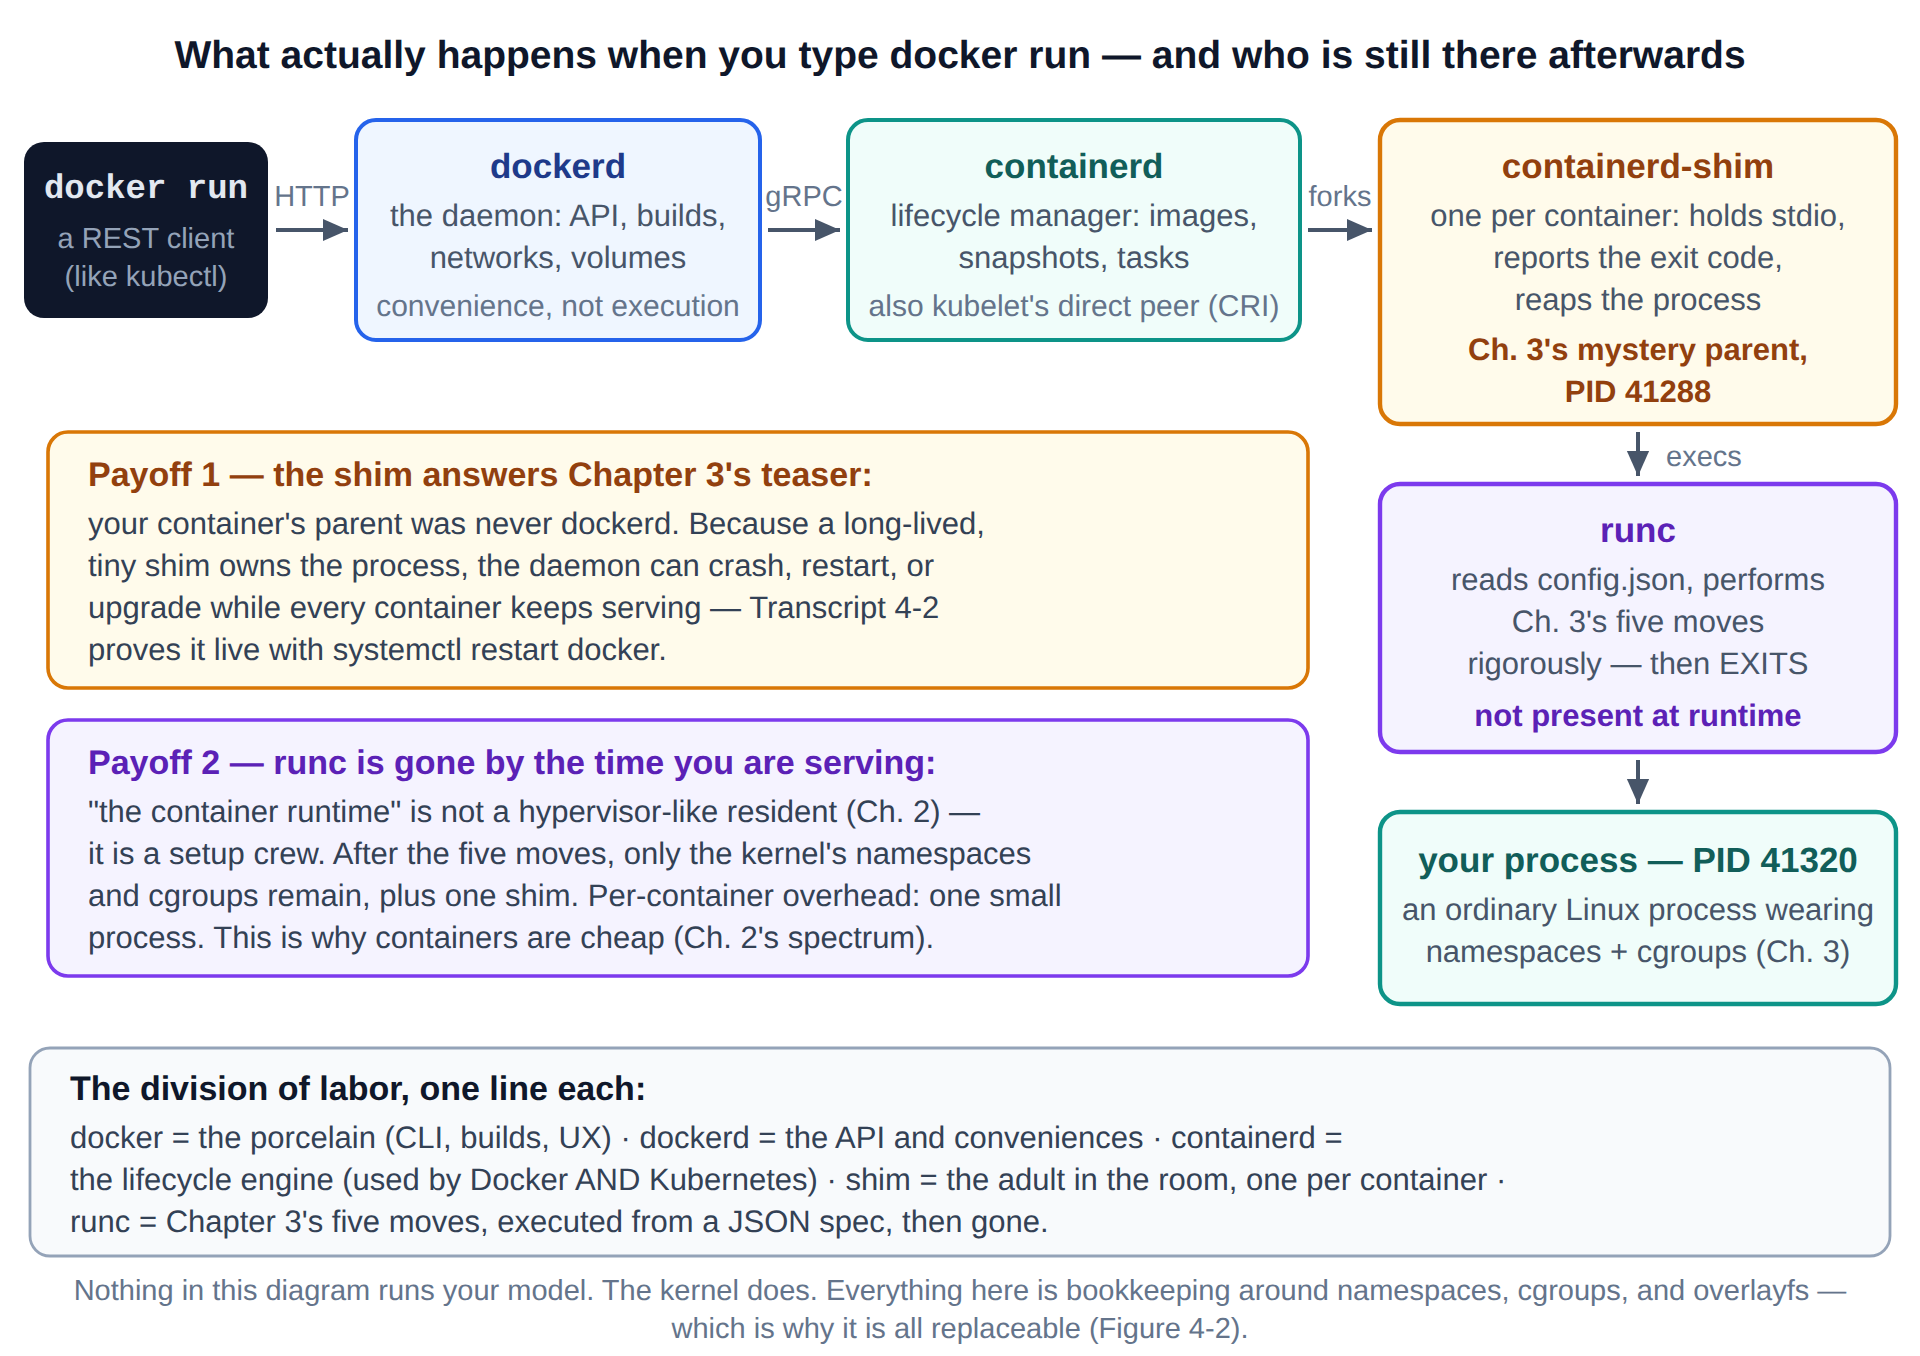
\includegraphics{figures/fig4-1_flow.png}}\\[3pt]
  \figcaption{그림 4-1  docker run의 흐름과 이후 남는 구성 요소. CLI와 데몬은 장부를 정리하고, runc는 제3장의 다섯 단계을 수행한 뒤 종료한다. 컨테이너마다 shim 하나가 남아 꼭 붙들어야 할 것을 맡는다.}
\end{tbbfigure}

\begin{tbbfigure}
  \adjustbox{max width=0.94\linewidth,max totalheight=0.46\textheight}{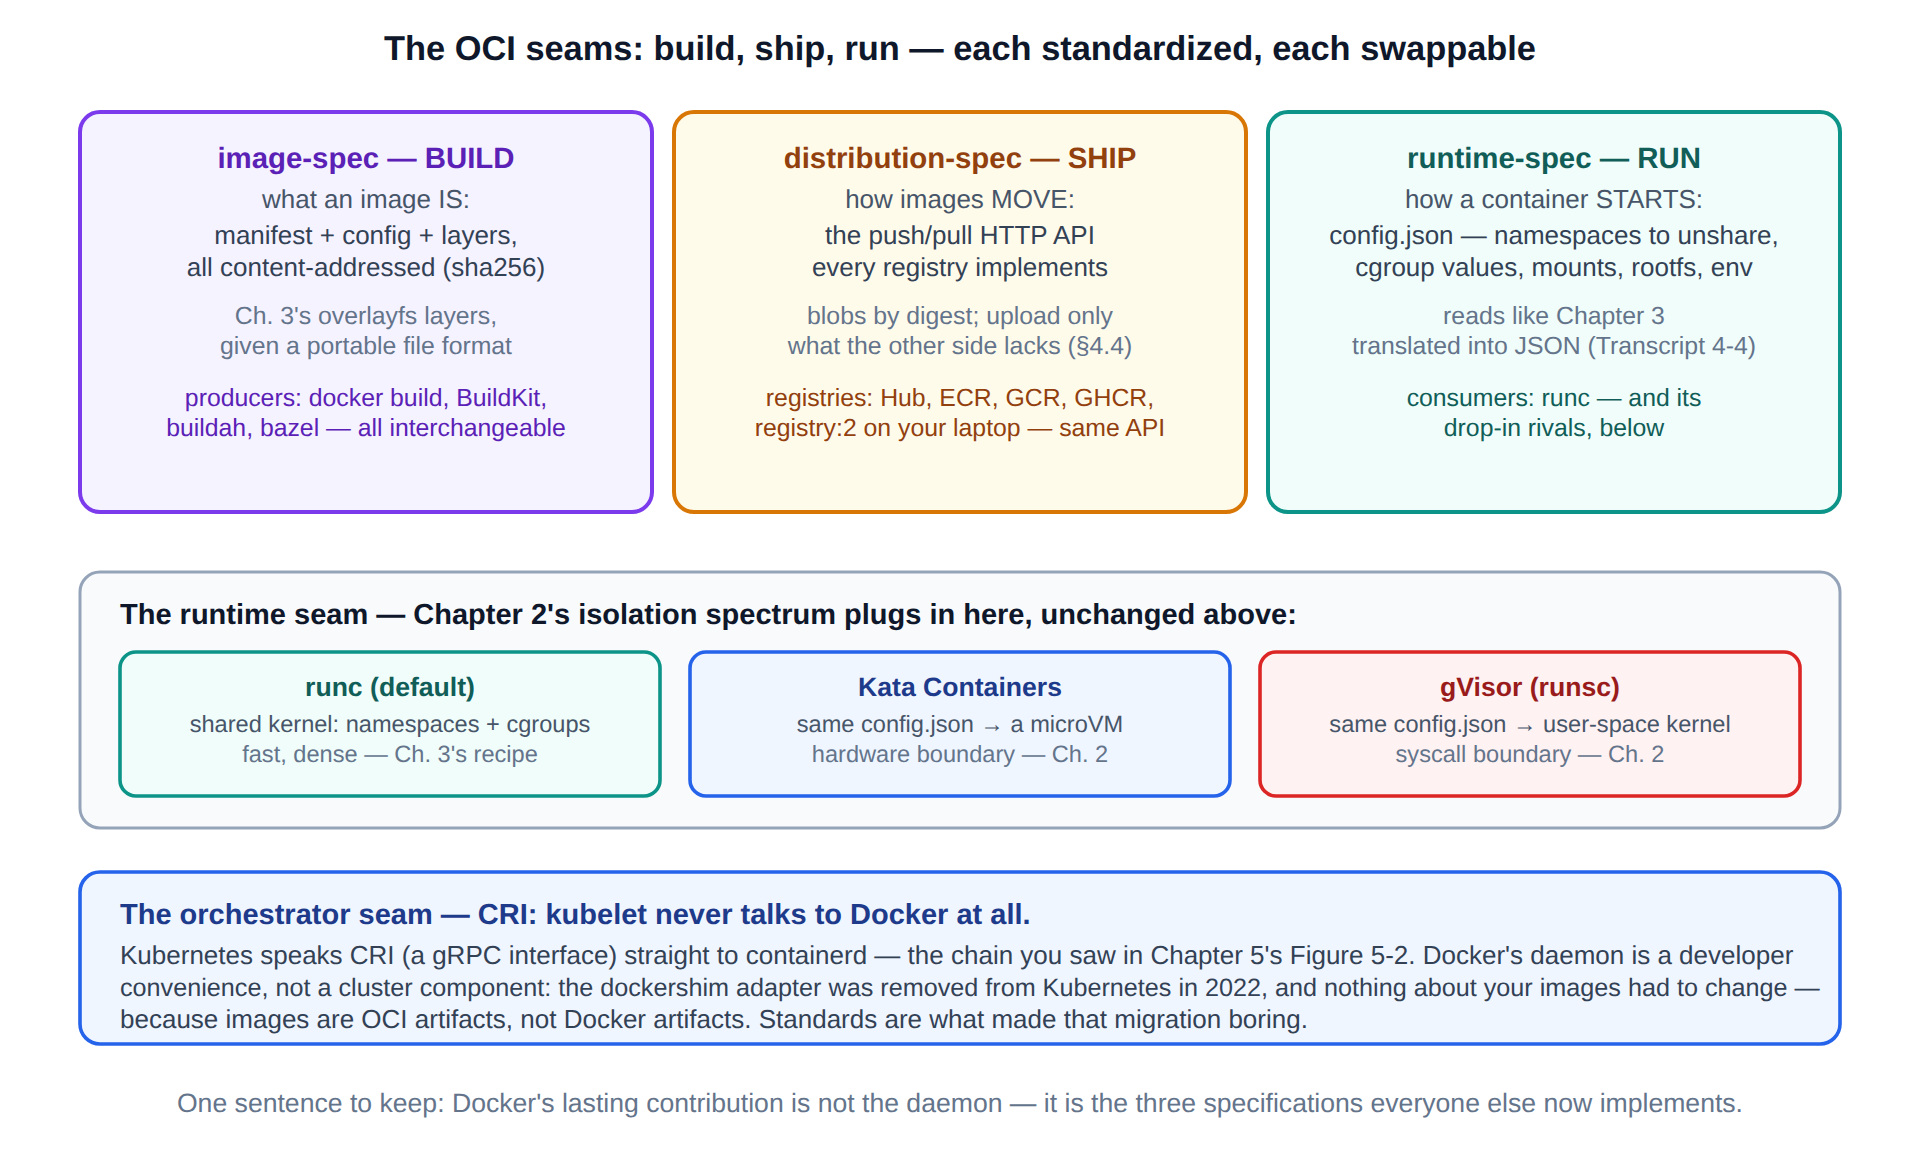
\includegraphics{figures/fig4-2_oci.png}}\\[3pt]
  \figcaption{그림 4-2  OCI 접합부. 빌드, 배포, 실행이 서로 다른 규격이므로 빌더·레지스트리·런타임을 독립적으로 교체할 수 있고, kubelet에는 Docker가 전혀 필요 없다.}
\end{tbbfigure}

\begin{calloutbox}{tbbpurple}{tbbpurplefill}
{\normalsize\bfseries\color{tbbpurple}생각해 보기}\par\vspace{3pt}
\begin{tbbitemize}
  \item 스택의 구성 요소(dockerd, containerd, shim, runc)를 장애가 서빙 플릿에 미치는 피해가 큰 순서대로 정렬하고, 각 구성 요소가 보유한 상태나 책임을 근거로 설명하라. 왜 아키텍처가 가장 작은 프로그램을 프로세스에 가장 가까이 두는지 답에서 드러나야 한다.
  \item Kata는 런타임 접합부에서 microVM으로 교체되며 "위쪽은 하나도 바뀌지 않는다." 제2장과 제3장을 바탕으로 워크로드에서 조용히 바뀌는 두 가지를 찾아라. 커널의 정체, /proc 내용, 장치 접근을 생각해 보자. 접합부는 계약을 표준화할 뿐 물리 법칙을 같게 만들지는 않는다.
  \item dockershim 제거는 거의 아무것도 깨뜨리지 않았지만 일부 팀에서는 \textit{무언가}가 깨졌다. 모든 노드에 Docker 데몬이 존재한다고 가정한 워크플로가 무엇인지 추론하라. CI 파드(Pod) 안의 docker build와 docker.sock 마운트를 단서로 삼고 OCI 네이티브 대안을 찾아보자.
\end{tbbitemize}
\end{calloutbox}

\section{엔지니어링 결과물로서의 이미지: 계층, 다이제스트, Dockerfile}

제3장에서는 overlayfs의 동작, 곧 읽기는 아래 계층으로 내려가고 쓰기는 위로 복사하며 삭제는 whiteout을 남긴다는 원리와 중복 제거·캐시·콜드 스타트 풀이라는 경제성을 배웠다. 이 절에서는 메커니즘을 \textbf{결과물}로 바꾼다. 정확히 무엇을 push하고, 어떻게 이름을 붙이며, 프로덕션에서 잘 동작하도록 어떻게 작성할까? 실제 이미지를 분해하는 데서 시작하자(그림 4-3).

\begin{terminalbox}
\begin{Verbatim}[breaklines=true,breakanywhere=true,fontsize=\small,formatcom=\color{tbbtermfg},codes=\tbbcodeactive]
$ docker build -t model-server:v1 . && docker images model-server
REPOSITORY     TAG   IMAGE ID       SIZE
model-server   v1    9f2c4a01be77   2.4GB
$ docker image inspect model-server:v1 --format \
    '{{.Architecture}} {{len .RootFS.Layers}} layers'
amd64 9 layers
$ docker history model-server:v1 --format "{{.Size}}\t{{.CreatedBy}}" | head -5
40kB    COPY serve.py /app/serve.py
1.9GB   RUN pip install -r requirements.txt
0B      WORKDIR /app
120MB   FROM python:3.11-slim
# every Dockerfile step that touched the filesystem = one layer,
# stackable and shippable exactly as Chapter 3 described.
\end{Verbatim}
\end{terminalbox}
\figcaption{터미널 기록 4-4  이미지를 분해했다. 파일 시스템을 건드리는 Dockerfile 단계는 계층과 일대일로 대응하며, 결과물의 정체는 친숙한 이름이 아니라 다이제스트다.}

구조적으로 OCI 이미지는 세 종류의 객체로 이루어지며, 각 이름은 바이트의 sha256이다. \textbf{매니페스트}는 작은 루트 문서로 \textbf{설정} 하나와 N개의 \textbf{계층} 다이제스트를 나열한다. 설정에는 runc에 전달할 env, \code{Cmd}, \code{User}, 노출 포트 같은 런타임 정보와 순서가 있는 계층 목록이 들어 있다. 계층은 제3장에서 본 읽기 전용 overlayfs 층을 압축한 tarball이다. 이 구조의 무게를 떠받치는 설계 선택은 \textbf{콘텐츠 주소 지정}이다. 모든 객체의 이름이 곧 해시이므로 몇 개의 이미지가 공유하든 동일한 계층은 한 번만 저장하고 전송한다(중복 제거). \code{sha256:22...}를 캐시한 머신은 누가 만들었는지 묻지 않고 절대적으로 신뢰할 수 있다. 서로 만난 적 없는 머신 사이에서도 계층 캐시가 작동하는 이유다. 무엇이든 변조하면 이름이 바뀐다(무결성). 반대로 \code{:v7} 같은 \textbf{태그}는 불변 세계를 가리키는 \textit{가변 포인터}, 즉 누군가 옮길 수 있는 별명이다. 운영 규칙은 자연스럽다. 사람은 태그로 말하지만 \textbf{배포는 다이제스트를 고정}한다(\code{image@sha256:aa41f9...}). 또는 레지스트리가 강제하는 불변 태그를 쓴다. 제6장에서 모델 버전에 같은 규율을 적용했는데, 이 책이 그 규율을 처음 배운 곳이 여기다.

\begin{tbbfigure}
  \adjustbox{max width=0.94\linewidth,max totalheight=0.46\textheight}{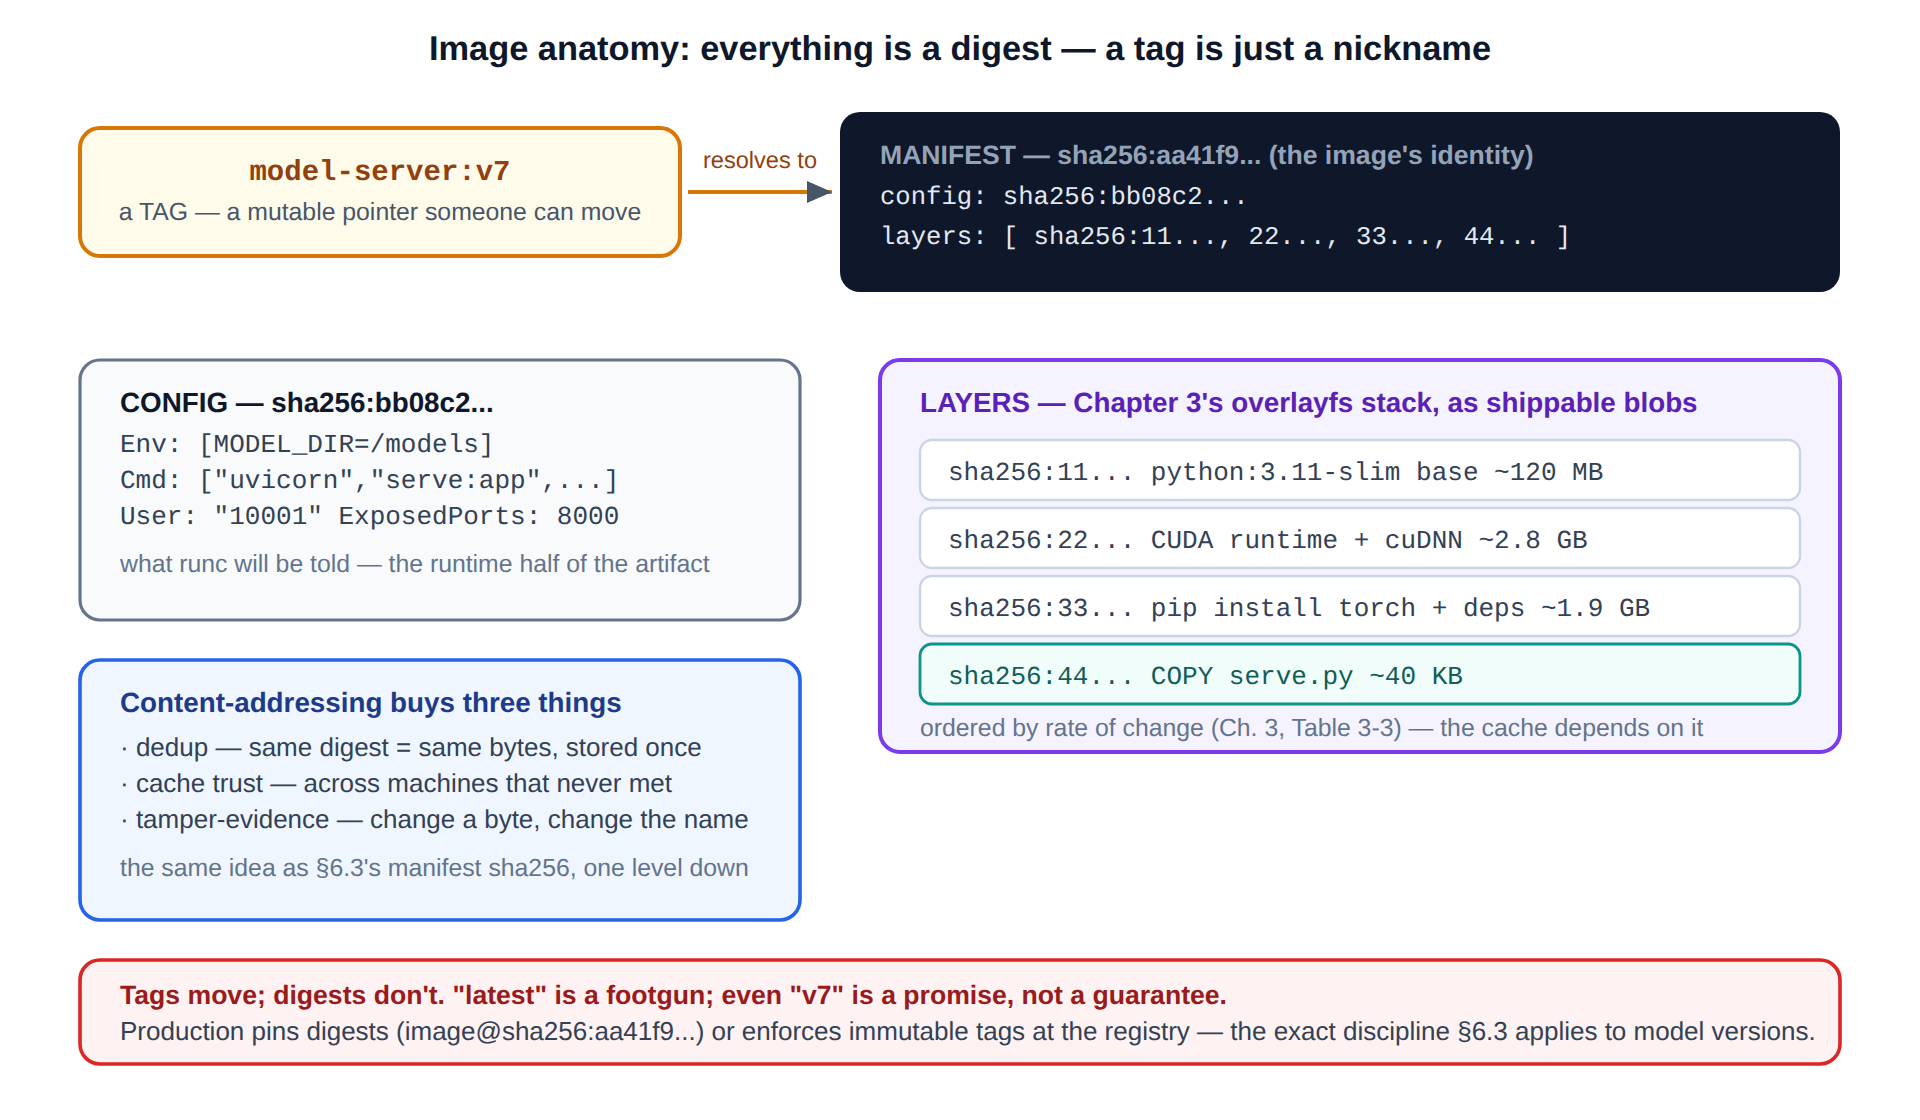
\includegraphics{figures/fig4-3_image.png}}\\[3pt]
  \figcaption{그림 4-3  이미지의 구조. 매니페스트가 설정과 계층을 가리키며 모든 것이 콘텐츠 주소로 식별된다. 태그는 바뀔 수 있는 별명이고 다이제스트는 정체다. 프로덕션 배포는 후자를 고정한다.}
\end{tbbfigure}

\subsection*{한 줄씩 설계하는 Dockerfile}

이미지를 작성하는 순간 이 책에서 쌓은 교훈이 파일 하나로 모인다. 아래는 실습 모델 서버의 Dockerfile이며, 모든 줄이 앞선 교훈을 증거와 함께 다시 불러온다. 그림 4-4에 전체 주석을 달았다.

\begin{terminalbox}
\begin{Verbatim}[breaklines=true,breakanywhere=true,fontsize=\small,formatcom=\color{tbbtermfg},codes=\tbbcodeactive]
# ---- stage 1: builder - compilers live here, and die here ----
FROM python:3.11 AS builder
COPY requirements.txt .
RUN pip install --prefix=/venv -r requirements.txt

# ---- stage 2: runtime - what actually ships ----
FROM python:3.11-slim
COPY --from=builder /venv /venv         # deps: change monthly
ENV PATH=/venv/bin:$PATH
RUN useradd -u 10001 serve
USER 10001                              # non-root (Ch. 3)
COPY serve.py /app/serve.py             # code: changes DAILY - last!
EXPOSE 8000
CMD ["uvicorn", "serve:app", "--host", "0.0.0.0", "--port", "8000"]
#   ^^ EXEC form: the server IS PID 1; SIGTERM lands (Ch. 3's bug)
\end{Verbatim}
\end{terminalbox}
\figcaption{터미널 기록 4-5  실습 Dockerfile. 순서로 제3장의 캐시 경제성을 구현하고, 다단계 빌드로 빌드 시점과 실행 시점 의존성을 분리하며, 마지막 줄로 제3장의 CMD 형식 버그를 영구히 고친다.}

가치의 대부분은 세 결정에서 나온다. \textbf{변경 빈도에 따른 순서}는 제3장의 표 3-3을 실행 가능하게 만든다. 천천히 바뀌는 베이스와 의존성은 아래에, 매일 바뀌는 \code{serve.py}는 마지막에 둔다. 그러면 매일 빌드할 때 40 KB짜리 마지막 계층만 새로 만들고 나머지는 모두 재사용한다. §4.4에 따라 매일의 \textit{push와 pull}도 KB만 움직인다. 여기서 중요한 결론이 하나 나온다. \code{COPY requirements.txt}와 \code{pip install}은 모든 \code{COPY . .}보다 \textit{앞에} 와야 한다. 전체 트리를 먼저 복사하면 코드 편집 하나가 의존성 계층을 무효화해 빌드마다 20분을 쓰게 된다. \textbf{.dockerignore}도 짝을 이룬다. 이미지에 들어오지 않는 빌드 컨텍스트는 캐시를 무효화할 수 없다. \code{.git}, 데이터셋, 제6장에서 다룰 로컬 모델 가중치를 제외하자. \textbf{다단계 빌드}는 실재하는 딜레마를 해결한다. 과학 계산 Python 패키지를 \textit{설치}하려면 약 1.9 GB의 컴파일러와 헤더가 필요하지만 실행할 때는 전혀 필요 없다. 1단계는 전체 도구 모음으로 \code{/\allowbreak venv}에 설치하고 2단계는 슬림 베이스에 \code{/\allowbreak venv}만 복사한다. 빌드 의존성이 실행 페이로드에서 빠져 CPU 실습 이미지는 2.4 GB에서 약 610 MB로 줄어든다. 마지막은 \textbf{PID 1 정확성과 비루트 실행}이다. exec 형식 \code{CMD}는 서버를 PID 1로 만들어 SIGTERM이 실제로 도달하게 한다. 제3장의 롤아웃, 제5장의 드레이닝, 제6장의 502 정렬이 한 줄에서 결실을 본다. \code{USER 10001}은 애플리케이션이 침해되어도 공격자가 비특권 사용자에 머물게 한다. 컨테이너 탈출의 피해를 줄이는 제3장의 교훈을 빌드 시점에 적용한 것이다.

\begin{tbbfigure}
  \adjustbox{max width=0.94\linewidth,max totalheight=0.46\textheight}{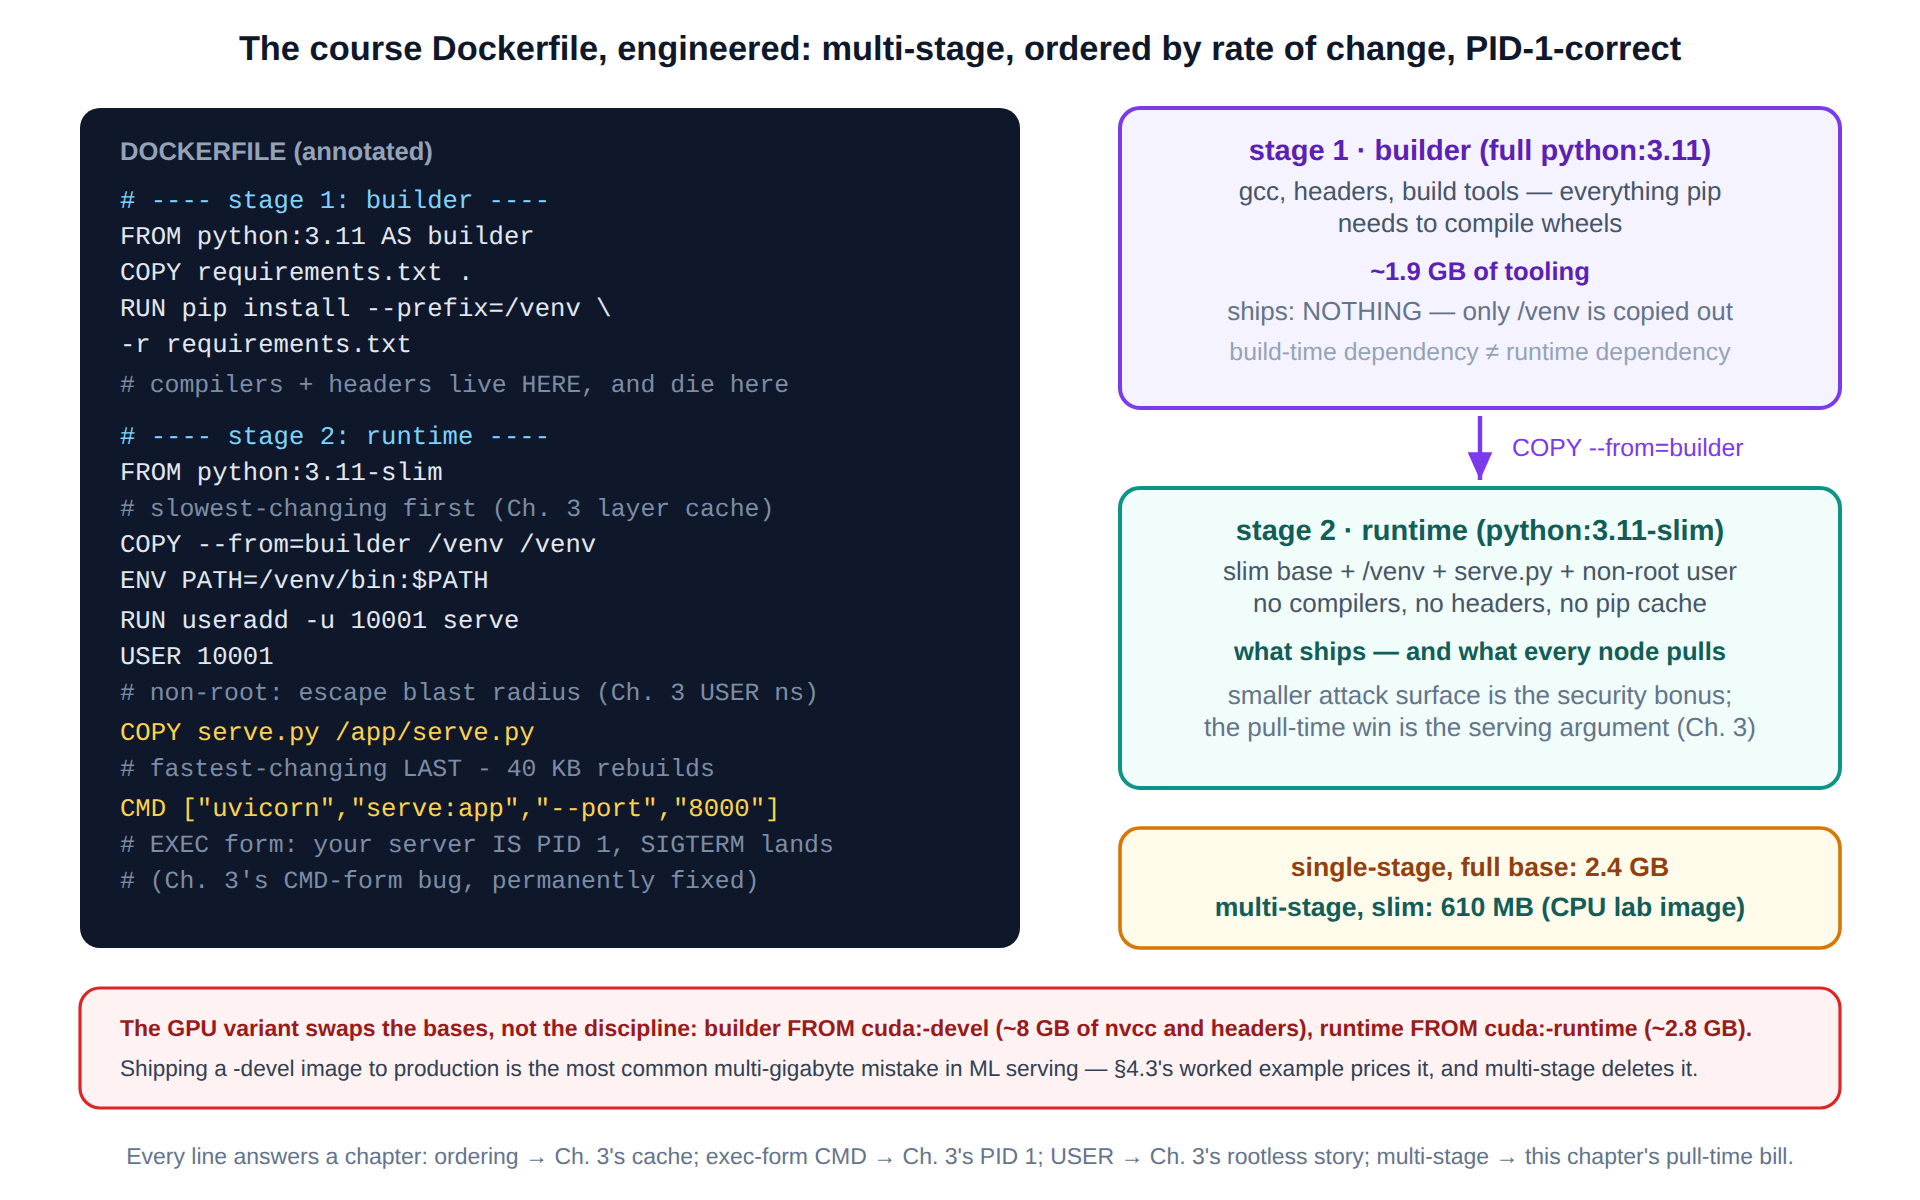
\includegraphics{figures/fig4-4_dockerfile.png}}\\[3pt]
  \figcaption{그림 4-4  설계된 Dockerfile. 다단계 빌드는 1.9 GB 도구 모음을 610 MB 결과물과 분리하고, 순서는 캐시를 보호하며, CMD와 USER 줄은 제3장의 교훈을 빌드에 얼려 넣는다.}
\end{tbbfigure}

\subsection*{GPU판: 가격표가 붙은 CUDA 태그 동물원}

GPU 서빙 이미지도 같은 규율을 따르지만 중요한 선택이 하나 더 있다. \textbf{어떤 CUDA 베이스를 쓸 것인가?} NVIDIA는 CUDA 버전마다 세 형태를 제공한다. \code{base}에는 드라이버와 맞닿는 라이브러리만 있고, \code{runtime}에는 CUDA 런타임과 cuDNN처럼 프레임워크를 \textit{실행}할 때 필요한 라이브러리가 더해진다. \code{devel}에는 nvcc, 헤더, 정적 라이브러리처럼 \textit{컴파일}할 때 필요한 약 8 GB의 도구가 추가된다. "개발 환경에서 됐으니까"라는 이유로 \code{devel}을 프로덕션에 보내는 실수가 반복되어 GB 단위 낭비를 만든다. 다단계 패턴은 올바른 선택을 기계적으로 만든다. \code{devel} 빌더 단계에서 커스텀 커널을 만들고, 최종 단계에는 \code{runtime}을 보낸다. 다음 계산 예시에서 차이에 가격표를 붙여 보자.

\begin{calloutbox}{tbbamber}{tbbamberfill}
{\normalsize\bfseries\color{tbbamberdark}계산 예시 — pull 시간과 비용으로 따진 이미지 다이어트}\par\vspace{3pt}
GPU 서빙 이미지를 세 방식으로 만든다. 용량은 대표값이며 제3장에서 계산한 유효 속도 100–250 MB/s로 pull한다.

\begin{tbbitemize}
  \item \textbf{단순형:} cuda:-devel 위의 단일 단계, pip보다 COPY가 먼저 오는 역전 구조로 \textbf{9.8 GB}다. 새 노드의 pull은 40–100 s가 걸리고, 역전 때문에 의존성 계층이 무효화되어 \textit{모든 코드 배포}마다 4 GB를 다시 보낸다.
  \item \textbf{순서 개선형:} 같은 베이스에 계층 순서만 바로잡는다. 첫 pull은 여전히 9.8 GB지만 코드 배포는 약 40 KB만 움직인다. 두 줄을 옮겨 문제의 절반을 해결했다.
  \item \textbf{설계형:} 다단계 빌드의 최종 단계를 cuda:-runtime으로 만든 \textbf{3.1 GB} 이미지다. 새 노드 pull은 12–31 s다. 12주 차의 콜드 스타트 항목은 약 3분의 1이 되고, 이미지 버전마다 노드 디스크를 약 7 GB 절약하며, 레지스트리 저장소와 송신 비용도 비례해 줄어든다.
\end{tbbitemize}

플릿 규모에서는 효과가 곱해진다. 새 노드 20대 × (9.8 − 3.1) GB = \textbf{플릿 전체의 콜드 pull 한 번당 레지스트리 트래픽 134 GB 절감}이다. 오토스케일링으로 노드를 늘릴 때마다 약 3배 빠르게 끝난다. 서버도 모델도 하드웨어도 같고 Dockerfile 하나만 다르다.
\end{calloutbox}

\vspace{3.0pt}

마지막으로 경계를 하나 그어야 한다. 결과물에 무엇을 넣을지 결정하는 경계다. 이미지는 runtime과 cuDNN 같은 CUDA \textbf{사용자 공간}을 담지만 \textbf{드라이버}는 절대 담지 않는다. 드라이버는 호스트의 속성이며 시작할 때 주입된다(§4.5). 제3장과 제6장에서 보았듯 \textbf{모델 가중치도 담지 않는다.} 모델 저장소에 두고 부팅할 때 불러온다. 그러면 이미지에는 코드, 의존성, 설정만 남는다. 코드와 같은 주기로 바뀌고 코드와 같은 리뷰 절차를 거쳐야 하는 부분, 바로 이미지가 담아야 할 내용이다.

\begin{calloutbox}{tbbpurple}{tbbpurplefill}
{\normalsize\bfseries\color{tbbpurple}생각해 보기}\par\vspace{3pt}
\begin{tbbitemize}
  \item 동료가 "모든 파일을 사용할 수 있게" Dockerfile 세 번째 줄에 COPY . /app을 넣는 빠른 수정을 제안했다. 빌드 시간, push 크기, 노드 pull, 12주 차 오토스케일러에 미치는 결과를 차례로 추적한 뒤, 두 줄을 옮기고 .dockerignore를 추가해 고쳐라.
  \item exec 형식 CMD 한 줄이 제3장, 제5장, 제6장에서 모두 보상받는 이유는 무엇인가? 각 장의 메커니즘을 이름 붙이고, 셸 형식을 쓰면 롤아웃·드레인(drain)·로드 밸런서에서 구체적으로 무엇이 깨지는지 설명하라.
  \item 다단계 빌드는 빌드 시점과 실행 시점 의존성을 분리한다. 한 계층 위의 모델 서빙에서 대응하는 사례를 들어라. §6.3의 모델 저장소는 무엇을 분리하며, "학습 컨테이너가 트래픽을 서빙한다"가 "devel 이미지를 배포한다"와 같은 실수인 이유는 무엇인가?
\end{tbbitemize}
\end{calloutbox}

\section{레지스트리: 콘텐츠 주소 기반 배포}

레지스트리는 겉보기에는 맥 빠질 만큼 단순하다. OCI distribution-spec을 구현한 HTTP 서비스로, 계층·설정·매니페스트 블롭을 다이제스트별로 저장했다가 돌려준다. Docker Hub, ECR, GCR, GHCR, 실습에서 실행할 \code{registry:2} 컨테이너는 \textit{같은 API}를 노출한다. 그래서 어느 곳에서든 \code{docker push}와 kubelet의 이미지 pull이 똑같이 작동한다. 블롭 자체는 보통 객체 스토리지에 놓이며 제6장에서 이 사실을 하나의 계약으로 다룬다. 흥미로운 엔지니어링은 저장소가 아니라 \textbf{대화}에 있다. push와 pull은 방향만 반대인 같은 협상이다. \textit{"여기 매니페스트가 있다. 이 중 없는 다이제스트가 무엇인가?"} 없는 블롭만 이동한다. 중복 제거는 최적화가 아니라 프로토콜 자체다(그림 4-5).

\begin{terminalbox}
\begin{Verbatim}[breaklines=true,breakanywhere=true,fontsize=\small,formatcom=\color{tbbtermfg},codes=\tbbcodeactive]
$ docker tag model-server:v1 localhost:5000/team/model-server:v1
$ docker push localhost:5000/team/model-server:v1
a1b2c3d4e5f6: Pushed        # 120MB  base (first push: everything moves)
b2c3d4e5f6a1: Pushed        # 1.9GB  deps
c3d4e5f6a1b2: Pushed        # 40kB   serve.py
v1: digest: sha256:aa41f9... size: 2415
# now change one line of serve.py, rebuild as :v2, push again:
$ docker build -q -t localhost:5000/team/model-server:v2 . && \
    docker push localhost:5000/team/model-server:v2
a1b2c3d4e5f6: Layer already exists
b2c3d4e5f6a1: Layer already exists
f6a1b2c3d4e5: Pushed        # 40kB - the only bytes that moved
v2: digest: sha256:bc52a0... size: 2415
\end{Verbatim}
\end{terminalbox}
\figcaption{터미널 기록 4-6  프로토콜이 작동하는 모습. 다른 다이제스트가 모두 "이미 존재"하므로 두 번째 push는 40 KB만 움직인다. pull도 대칭이며, 따라서 일상적인 배포 비용은 낮지만 콜드 노드의 비용은 높다.}

pull 쪽을 보면 경제성이 완성된다. 노드는 containerd 스냅숏 형태의 \textbf{로컬 계층 캐시}를 유지한다. \code{v1}을 서비스하던 노드에 \code{v2}를 pull하면 40 KB 계층 하나만 가져온다. 그래서 제5장의 롤링 업데이트(rolling update)는 이미 따뜻한 플릿에서 조용히 지나간다. 비싼 경우는 \textbf{새 노드}다. CUDA 크기의 이미지는 모든 것을 한 번 내려받아야 하므로 제3장에서 계산한 25–60 s가 든다. 병적인 경우는 \textbf{풀 폭풍}이다. 확장이나 플릿 전체 배포가 여러 새 노드를 동시에 건드려 GB에 노드 수를 곱한 트래픽을 하나의 레지스트리 경로로 보낸다. 가장 급한 순간에 일어난다. 12주 차에는 오토스케일링의 콜드 스타트 세금으로 다시 만난다. 대응은 §4.3의 이미지 다이어트, 노드 이미지 캐시와 사전 pull, 같은 지역의 풀스루 미러, 더 나아가 지연 로딩(lazy loading) 스냅쇼터 순이다. 터미널 기록이 push 끝마다 출력하는 \textbf{매니페스트 다이제스트}도 보자. 이 문자열이 배포 가능한 정체다. 태그는 움직이므로 제5장의 매니페스트는 다이제스트(\code{image@sha256:...})나 불변 태그를 참조해야 한다. "v2라는 이름의 \textit{무언가}를 배포했다"는 감사 기록이 아니다. 13주 차 파이프라인이 환경 사이에서 다이제스트를 승격하는 이유다.

\begin{tbbfigure}
  \adjustbox{max width=0.94\linewidth,max totalheight=0.46\textheight}{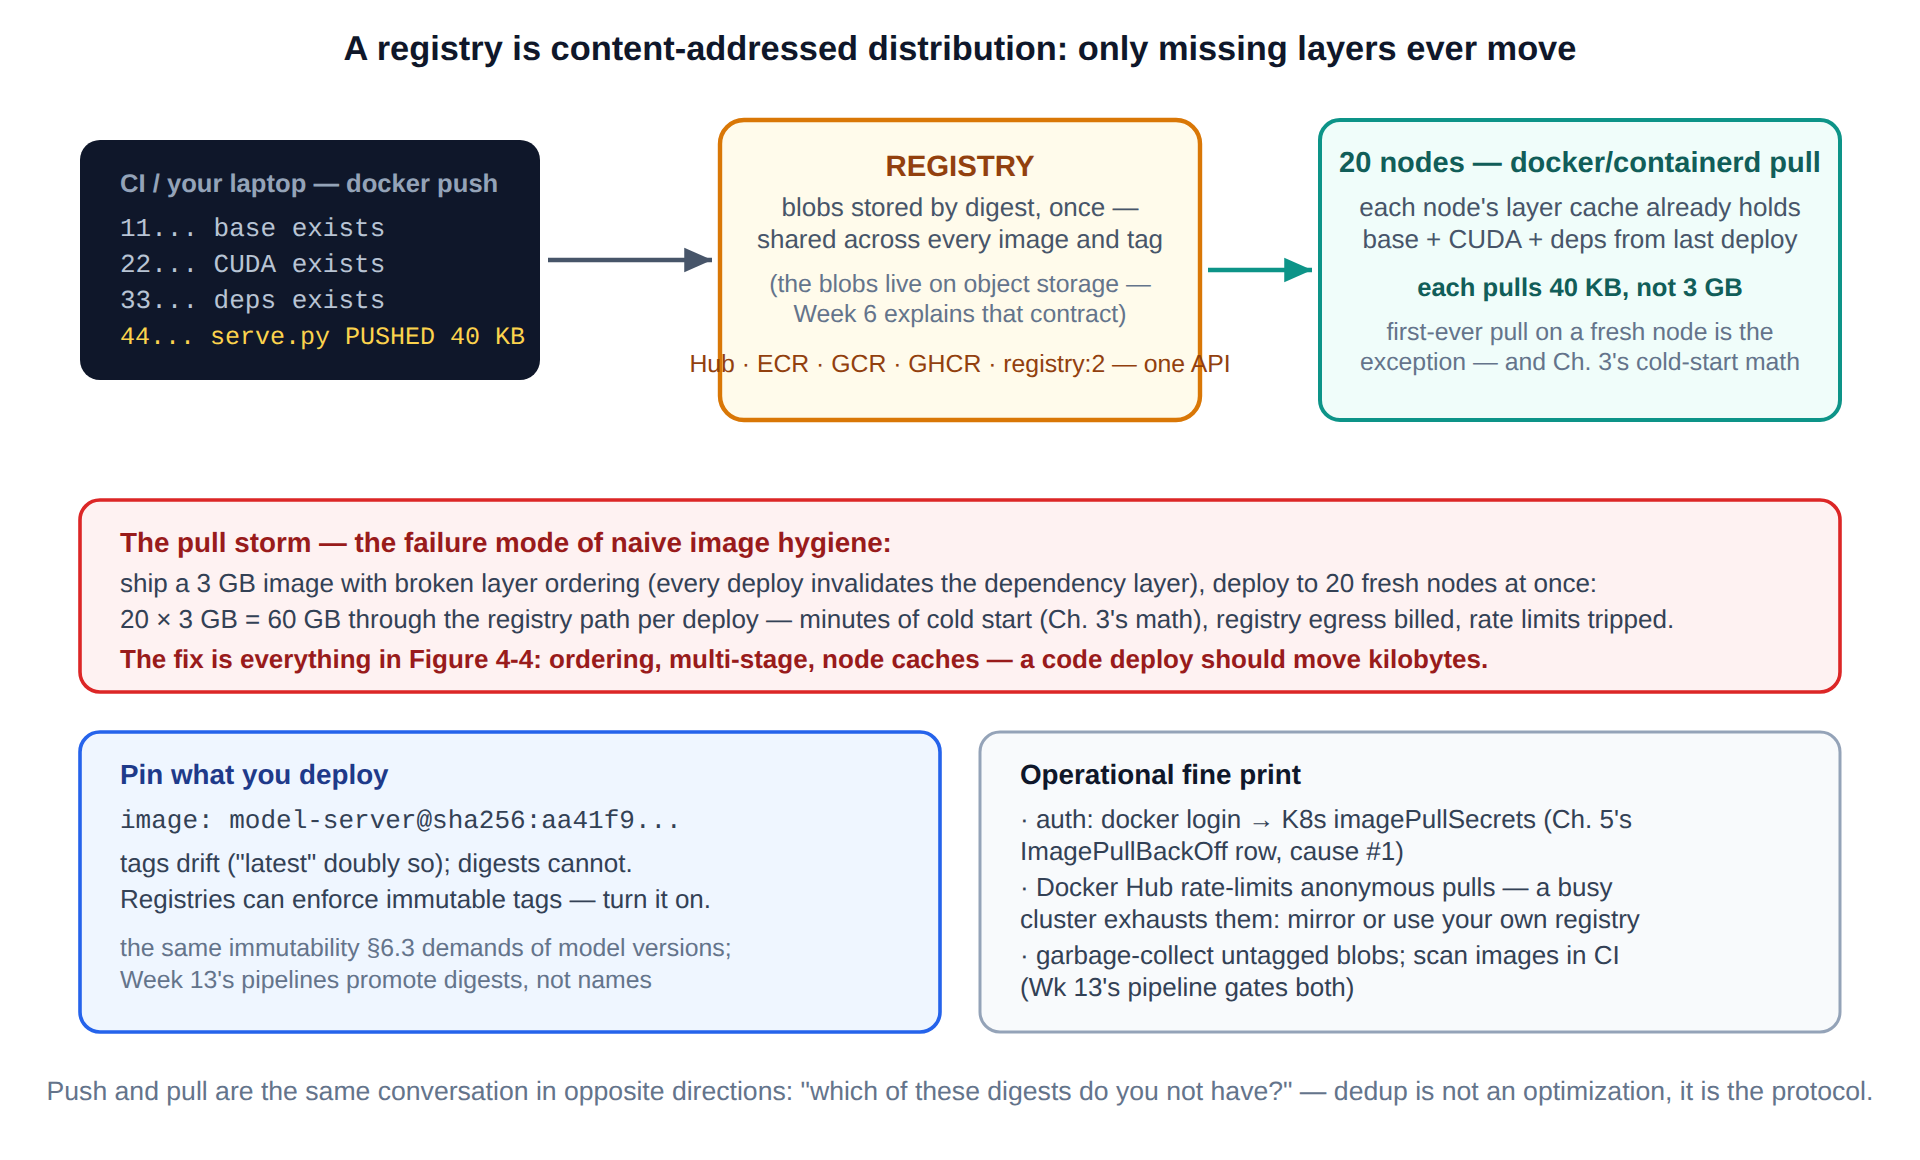
\includegraphics{figures/fig4-5_registry.png}}\\[3pt]
  \figcaption{그림 4-5  콘텐츠 주소 기반 배포. push와 pull은 없는 다이제스트만 움직이고, 노드 캐시는 코드 배포를 KB 단위로 만든다. 새 노드와 풀 폭풍은 별도로 설계해 피해야 할 비싼 예외다.}
\end{tbbfigure}

\subsection*{장애로 이어지는 운영상의 세부 사항}

\begin{tbbitemize}
  \item \textbf{인증.} \code{docker login}은 자격 증명을 저장하고, Kubernetes에는 같은 자격 증명을 \code{imagePullSecrets} 참조로 건네야 한다. 제5장의 ImagePullBackOff 행에 적힌 첫 번째 원인이다. 클라우드 레지스트리는 인스턴스/파드 IAM과 통합한다. 잘 구성한 클러스터의 노드는 정적 시크릿 없이도 비공개 이미지를 pull한다. 제6장의 키 없는 패턴이 다시 등장한다.
  \item \textbf{속도 제한.} Docker Hub의 익명 pull 제한은 작은 클러스터도 배포 도중 할당량을 다 쓸 만큼 엄격하다. \code{toomanyrequests: You have reached your pull rate limit}는 실제 장애 유형이다(§4.6). 구조적 해법은 "더 열심히 로그인"하는 것이 아니다. 의존하는 공개 베이스를 자체 레지스트리에 미러링하자. \code{registry:2}의 플래그 하나로 풀스루 캐시를 만들 수 있고, 업스트림 장애와 삭제에도 견딘다.
  \item \textbf{위생.} 태그는 쌓이고, 태그 없는 매니페스트와 주인 없는 블롭은 가비지 컬렉션 전까지 남는다. 레지스트리에 보존 정책이 있는 데는 이유가 있다. "GC를 한 번도 하지 않아 레지스트리 비용이 두 배가 됐다"는 분기마다 실제로 마주치는 황당한 비용 증가다. 보존 정책에 push 시 CVE를 검사하는 \textbf{스캐닝}을 함께 적용하자. 13주 차 파이프라인은 둘 모두를 관문으로 삼는다.
  \item \textbf{아키텍처.} 저장소는 같은 태그가 amd64와 arm64 이미지로 각각 해석되는 \textbf{다중 아키텍처 매니페스트 목록}을 담을 수 있다. Apple Silicon 노트북에서 \code{--platform} 없이 빌드하면 클라우드 노드가 arm64 전용 이미지를 pull하는 순간 §4.6의 \code{exec format error}를 만난다. \code{docker buildx --platform linux/\allowbreak amd64,linux/\allowbreak arm64}로 둘 다 게시하자. 노트북이 아니라 CI가 맡아야 할 일이다.
\end{tbbitemize}

\begin{calloutbox}{tbbpurple}{tbbpurplefill}
{\normalsize\bfseries\color{tbbpurple}생각해 보기}\par\vspace{3pt}
\begin{tbbitemize}
  \item 터미널 기록 4-6의 동작을 이용해 계산해 보자. 올바르게 계층화한 이미지를 따뜻한 노드 20대에 하루 6회 배포한다. 하루 레지스트리 트래픽을 추정한 뒤 §4.3의 COPY 순서 역전 버그가 있을 때 다시 계산하라. 제3장의 생각해 보기 문제에 배포 비용까지 더한 셈이다.
  \item 풀스루 미러는 같은 지역에 공개 이미지를 캐시한다. 서로 다른 세 가지 실패/비용 유형 가운데 무엇을 막아 주는지 나열하고, 새로 생기는 실패 하나도 찾아라.
  \item 13주 차 파이프라인은 환경마다 이미지를 다시 태깅("staging" → "prod")하지 않고 다이제스트를 승격해야 한다. 각 접근에서 생기는 구체적인 경합과 롤백(rollback) 시나리오를 제시하라.
\end{tbbitemize}
\end{calloutbox}

\section{GPU를 상자 안에 넣는 법}

이제 제2장부터 아껴 둔 질문, 강의계획서의 괄호 안 질문을 다룬다. \textit{cgroup은 왜 GPU 연산을 스케줄링할 수 없으며, 그렇다면 컨테이너는 어떻게 GPU를 사용하는가?} 먼저 컨테이너의 본질을 떠올리자(제3장). 프로세스 주위에 네임스페이스와 cgroup을 두지만 \textbf{아무것도 가상화하지 않는다.} 따라서 제2장의 virtio가 디스크를 VM 안에 에뮬레이션한 것처럼 GPU를 컨테이너 안에 흉내 낼 수 없다. 진짜 장치를 건네야 한다. 그 "진짜 장치"도 단일 부품이 아니라 단층선이 있는 \textit{스택}이다. 호스트에는 \textbf{커널 모듈}(\code{nvidia.ko})과 버전이 정확히 일치하는 \textbf{드라이버 사용자 공간 라이브러리}가 있고, 그 위에는 애플리케이션이 링크하는 런타임·cuDNN·프레임워크 등의 \textbf{CUDA 사용자 공간}이 있다. 이 단층선이 ML 이미지를 운반할 수 있게 하는 패키징 규칙을 결정한다. \textbf{이미지는 CUDA 사용자 공간을 담고, 호스트는 드라이버를 담으며, 이미지 안의 어떤 것도 특정 드라이버 빌드에 의존해서는 안 된다}(그림 4-6).

\begin{tbbfigure}
  \adjustbox{max width=0.94\linewidth,max totalheight=0.46\textheight}{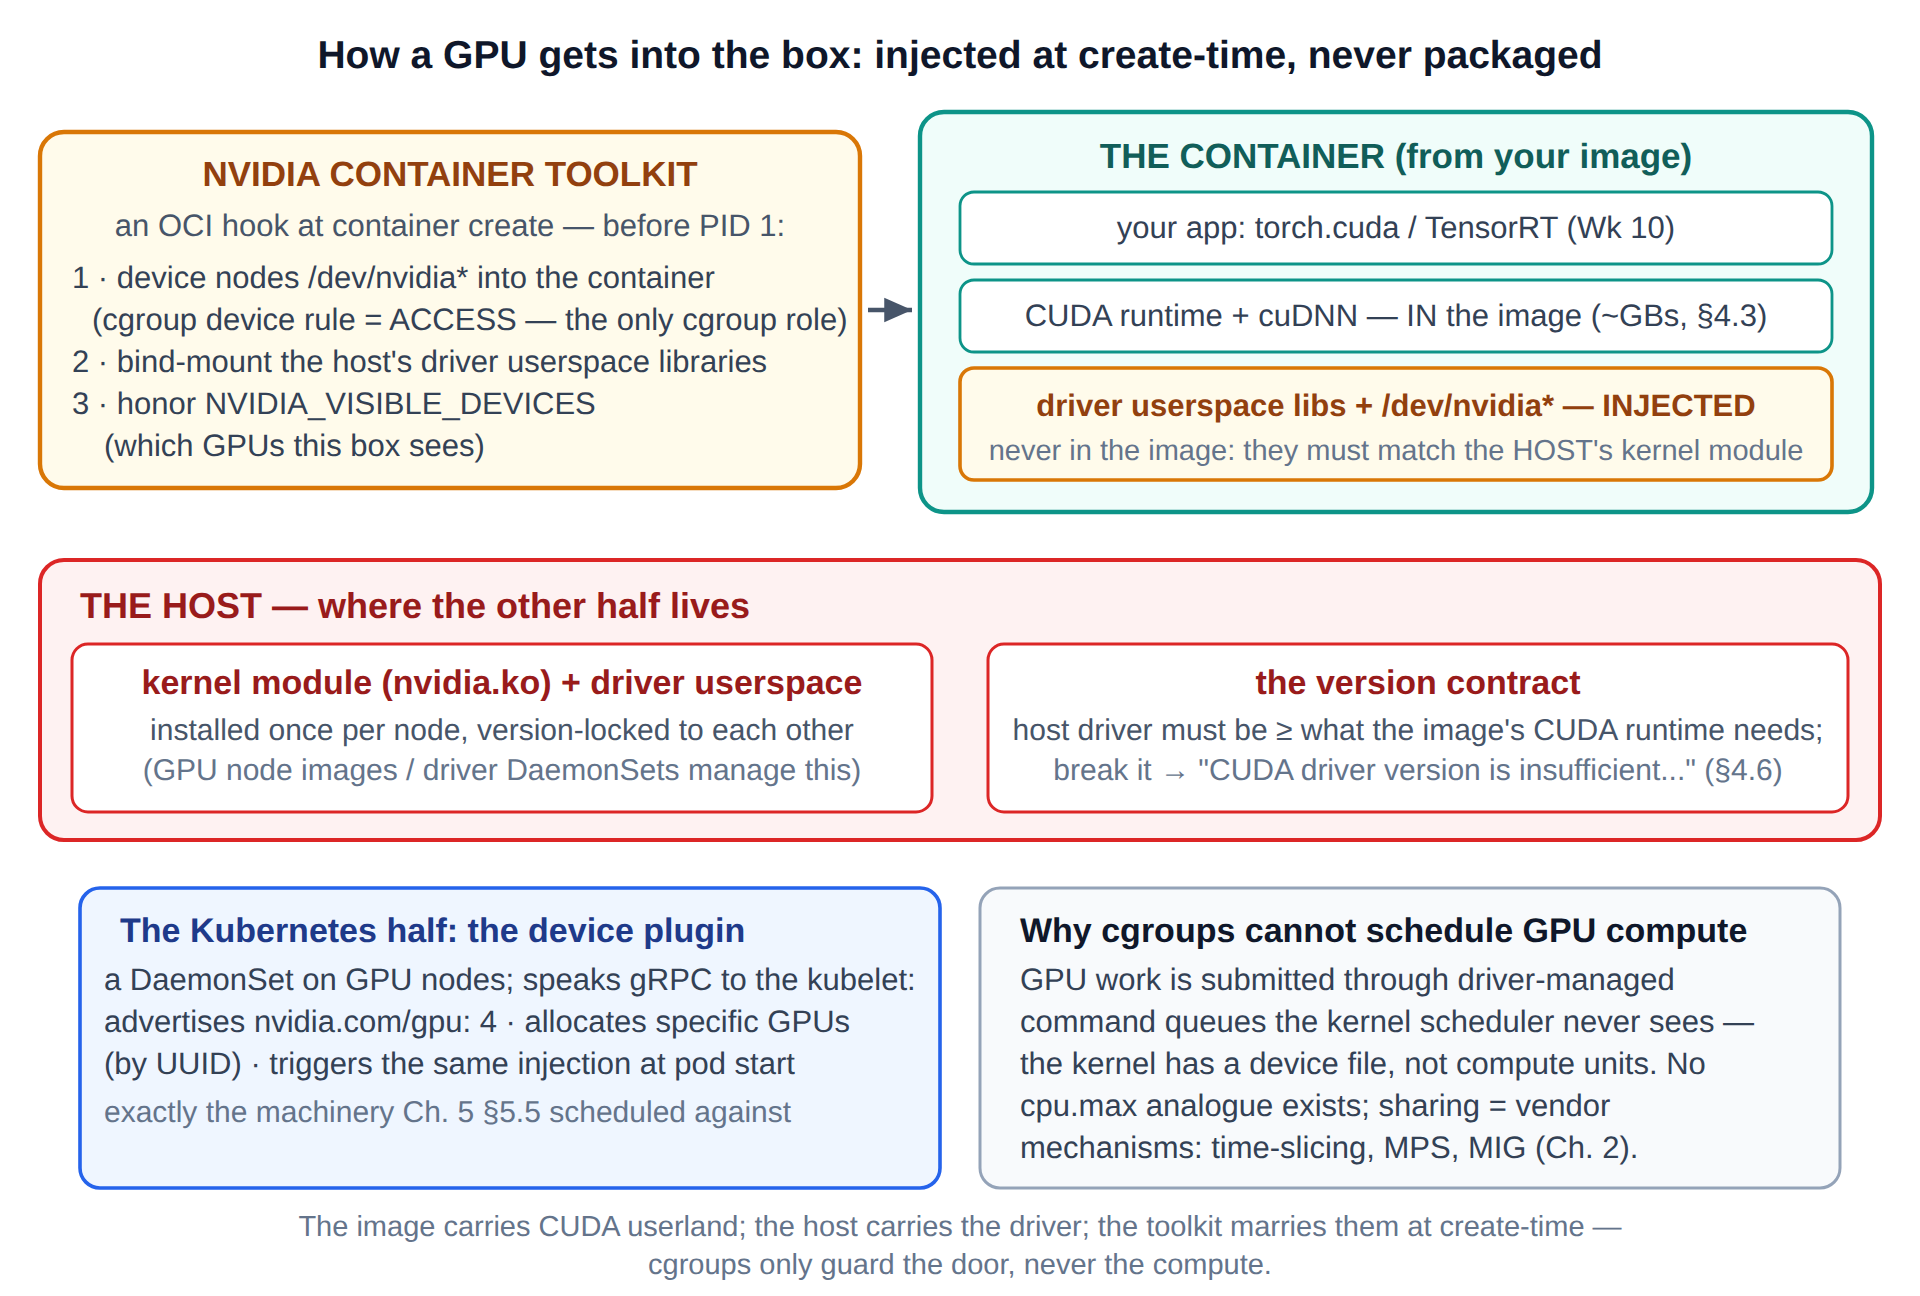
\includegraphics{figures/fig4-6_gpu.png}}\\[3pt]
  \figcaption{그림 4-6  GPU는 생성 시점에 들어온다. 툴킷의 OCI 훅이 장치 노드와 호스트의 드라이버 사용자 공간을 주입하고, 이미지에는 CUDA 사용자 공간만 들어 있다. cgroup은 문을 지키고 드라이버는 연산을 맡는다.}
\end{tbbfigure}

\subsection*{메커니즘: OCI 훅과 세 가지 주입}

\textbf{NVIDIA Container Toolkit}은 이 결합을 OCI 계층의 훅으로 구현한다. shim 런타임인 \code{nvidia-container-runtime}이 runtime-spec 묶음을 받아 수정한 뒤 평범한 runc에 넘긴다. 컨테이너 생성 시점, PID 1이 존재하기 전에 세 가지를 주입한다. 첫째는 \textbf{장치 노드}다. \code{/\allowbreak dev/\allowbreak nvidia0}, \code{/\allowbreak dev/\allowbreak nvidiactl}, \code{/\allowbreak dev/\allowbreak nvidia-uvm}이 컨테이너에 나타나고 cgroup의 \textit{장치 규칙}이 이를 허용한다. GPU 이야기 전체에서 cgroup이 관여하는 부분은 이것뿐이다. 파일을 열 수 있는지 허용/거부하는 일로, 제3장의 "접근 관문"이 구체화된 모습이다. 둘째, \textbf{드라이버 사용자 공간 라이브러리}를 호스트에서 바인드 마운트한다. \code{nvidia.ko}와 버전이 맞아야 하는 절반을 \code{nvidia.ko}와 같은 머신에서 가져오는 것이 핵심이다. 셋째, 환경 변수 \code{NVIDIA\_VISIBLE\_DEVICES}가 컨테이너에 보일 GPU를 선택한다. GPU 4개가 있는 노드가 서로 다른 컨테이너에 서로 다른 장치를 건네는 방식이다.

\begin{terminalbox}
\begin{Verbatim}[breaklines=true,breakanywhere=true,fontsize=\small,formatcom=\color{tbbtermfg},codes=\tbbcodeactive]
$ docker run --rm --gpus '"device=0"' nvidia/cuda:12.4-runtime nvidia-smi \
    --query-gpu=index,name,memory.total --format=csv,noheader
0, NVIDIA A10G, 23028 MiB
$ docker inspect $(docker ps -lq) --format '{{json .HostConfig.DeviceRequests}}'
[{"Driver":"nvidia","Count":0,"DeviceIDs":["0"],"Capabilities":[["gpu"]]}]
# and the injected mounts, visible like any other config:
$ docker inspect $(docker ps -lq) | grep -c "nvidia"
23        # device nodes + driver libs + env - all inspectable
# the failure mode, staged: an image whose CUDA is newer than the host driver:
$ docker run --rm --gpus all nvidia/cuda:99.9-runtime python3 -c "..."
CUDA driver version is insufficient for CUDA runtime version
# the version contract of Figure 4-6, breached on purpose (sec. 4.6).
\end{Verbatim}
\end{terminalbox}
\figcaption{터미널 기록 4-7  GPU 접근은 마법이 아니라 설정이다. HostConfig의 장치 요청, 주입된 노드와 마운트를 모두 inspect할 수 있다. 이미지의 CUDA가 호스트 드라이버보다 앞서면 고전적인 오류가 발생한다.}

\subsection*{Kubernetes 쪽 절반과 질문의 완전한 답}

클러스터에서는 발견과 할당이 한 계층 위로 올라간다. GPU 노드의 DaemonSet인 \textbf{디바이스 플러그인(device plugin)}은 kubelet과 gRPC로 통신한다. 노드 용량에 \code{nvidia.com/\allowbreak gpu: 4}를 알리고, GPU를 요청한 파드가 배치되면 UUID로 어떤 물리 장치를 허용할지 kubelet에 알려 준다. 이는 제5장의 스케줄러가 예산으로 사용한 바로 그 숫자다. 이어 kubelet의 CRI 호출이 방금 Docker에서 본 것과 같은 툴킷 주입을 촉발한다. 아래쪽에서는 새로운 일이 없다. Kubernetes는 변하지 않은 메커니즘 위에 재고 관리와 배치를 더한다. 제5장 §5.5의 "확장 리소스는 정수다"라는 문장의 기계실을 이제 들여다보았다.

이제 강의계획서가 물었던 \textit{왜}가 남는다. 커널은 자신이 볼 수 있는 것을 스케줄링한다. 실행 대기열을 소유하므로 CPU 시간을 보고 \code{cpu.max}로 버스트 중인 작업도 멈출 수 있다. 페이지 테이블을 소유하므로 메모리를 보고 \code{memory.max}로 할당을 거부할 수 있다. GPU 연산은 설계상 커널에 보이지 않는다. 사용자 프로세스는 \textbf{드라이버가 관리하는 명령 대기열}로 작업을 제출한다. 이 대기열은 사용자 공간에 직접 매핑되어 제출할 때 시스템 호출조차 하지 않는 경우가 많다. 다음에 실행할 작업은 GPU 자체의 엔진과 펌웨어가 고른다. 커널이 보는 GPU 전체는 열기를 허용하거나 거부할 수 있는 장치 파일일 뿐이다. cgroup 컨트롤러가 측정할 만한, 커널에 보이는 "GPU 시간" 단위가 없으므로 GPU 컨트롤러도 없다. 이 한 문장에서 이후 모든 내용이 따라온다. 공유는 대기열을 \textit{볼 수 있는} 드라이버와 하드웨어, 곧 \textbf{공급업체 계층}에서 제공해야 했다(제2장의 시간 분할, MPS, MIG). Kubernetes는 아래에서 강제할 수 없는 것을 약속하지 않으므로 GPU를 \textbf{나눌 수 없는 정수}로 스케줄링한다(제5장). 메모리에서 누린 OOM식 안전망은 VRAM에는 없다. 전부 쓰면 커널과 무관하게 제3장의 \textit{다른} OOM, 곧 잡아서 처리할 수 있는 CUDA 할당자 오류를 받는다.

\begin{calloutbox}{tbbblue}{tbbbluefill}
{\normalsize\bfseries\color{tbbblue}네 장에 걸친 GPU 이야기를 한곳에 모으기}\par\vspace{3pt}
\begin{tbbitemize}
  \item \textbf{제2장:} 하드웨어를 공유할 수 있지만 PCIe 패스스루, vGPU, 시간 분할, MPS, MIG 같은 공급업체 메커니즘만 가능하다.
  \item \textbf{제3장:} 커널은 GPU를 중재할 수 없다. cgroup GPU 컨트롤러는 없고 장치 파일 접근만 통제한다.
  \item \textbf{제4장(현재):} 따라서 접근은 \textit{주입}이다. OCI 훅이 생성 시점에 호스트 드라이버와 장치 노드를 이미지의 CUDA 사용자 공간에 결합하고, 디바이스 플러그인이 발견과 할당을 맡는다.
  \item \textbf{제5장:} 오케스트레이션은 GPU를 정수 확장 리소스로 다룬다. 분수도 오버커밋도 없고 requests = limits다. 분할 수요는 제2장의 메커니즘으로 돌아가며 12주 차에 운영 방법을 다룬다.
\end{tbbitemize}
\end{calloutbox}

\vspace{3.0pt}

\begin{calloutbox}{tbbpurple}{tbbpurplefill}
{\normalsize\bfseries\color{tbbpurple}생각해 보기}\par\vspace{3pt}
\begin{tbbitemize}
  \item 호스트의 드라이버 라이브러리를 이미지에 넣는 방식, 곧 "내 노드에서는 됐는데"가 왜 이식성 시한폭탄이 되는가? 이미지는 고정된 채 플릿의 노드 풀이 드라이버 버전을 올릴 때 벌어지는 일을 추적하라.
  \item NVIDIA\_VISIBLE\_DEVICES는 주입으로 강제한다. 허용받지 않은 장치는 컨테이너에 아예 보이지 않는다. 이를 제3장의 memory.max 강제 모델과 비교하라. 각 방식에서 가능한 실패는 무엇인가? 두 컨테이너에 \textit{같은} GPU를 허용하면 어떤 일이 생길지 생각해 보자.
  \item 이 절과 제2장을 바탕으로 "GPU 시간용 cgroup 컨트롤러를 만들자. 얼마나 어렵겠어?"라는 제안을 두 문단으로 기술적으로 반박하라. 커널이 보아야 하지만 볼 수 없는 것은 무엇이며, 측정은 대신 어느 계층에 있어야 하는가?
\end{tbbitemize}
\end{calloutbox}

\section{검시관처럼 컨테이너 읽기: inspect 현장 안내서}

징후, 원인, 첫 명령으로 정리하는 이 책의 현장 안내서 습관은 제3장의 종료 코드 하나에서 시작해 장마다 한 계층씩 자란다. Docker 계층에서는 도구 하나가 중심이다. \textbf{docker inspect}는 무엇을 \textit{실제로} 설정했고 무엇이 \textit{실제로} 일어났는지 플랫폼이 JSON으로 제출하는 선서 증언이다. 선언한 이미지·환경·상한·장치와 스택이 기록한 상태·종료 코드·OOM 플래그·재시작 횟수가 모두 들어 있다. 어떤 질문에 어느 필드가 답하는지 아는 것이 기술이다. 실습의 필수 연습이 가장 좋은 도입이다. 제3장의 첫 터미널 기록에서 시작한 고리를 닫기 때문이다.

\begin{terminalbox}
\begin{Verbatim}[breaklines=true,breakanywhere=true,fontsize=\small,formatcom=\color{tbbtermfg},codes=\tbbcodeactive]
$ docker run -d --name demo -m 512m --cpus 1 model-server:v1
$ docker inspect demo --format \
    'mem={{.HostConfig.Memory}} nanocpus={{.HostConfig.NanoCpus}}'
mem=536870912 nanocpus=1000000000     # your flags, recorded verbatim
$ PID=$(docker inspect demo --format '{{.State.Pid}}') && echo $PID
41320
$ CG=$(cat /proc/$PID/cgroup | cut -d: -f3) && \
    cat /sys/fs/cgroup$CG/memory.max /sys/fs/cgroup$CG/cpu.max
536870912                             # the SAME number, in the kernel
100000 100000                         # --cpus 1, in Ch. 3 grammar
# intent (inspect) == enforcement (cgroupfs): the ghostwriter, audited.
# this is Transcript 3-1 closed from both ends - and the lab's Part B.
\end{Verbatim}
\end{terminalbox}
\figcaption{터미널 기록 4-8  강의계획서가 요구한 감사. docker inspect는 기록된 의도를, cgroup 파일 시스템은 커널의 강제를 보여 준다. 제3장의 대필자가 이 장의 스택이므로 숫자가 일치한다.}

여섯 필드가 질문의 90\%에 답하므로 작은 JSON 지도를 기억하자. \textbf{.State}는 실행 중인지, 아니라면 \textit{어떻게 끝났는지} 알려 준다. \code{ExitCode}, \code{OOMKilled}, \code{Error}, 타임스탬프가 있다. 죽은 컨테이너는 서류가 딸린 시신이며 \code{docker logs}도 여전히 작동한다. 제5장의 \code{--previous} 비행 기록 장치 습관이 한 계층 아래에 있다. \textbf{.Config}는 \textit{이미지}가 말한 env, \code{Cmd}, \code{User}, 노출 포트다. \textbf{.HostConfig}는 \textit{운영자}가 말한 상한, 재시작 정책, 장치, 마운트, 포트 게시다. 의도와 현실이 다를 때 의도는 여기에 적혀 있다. \textbf{.GraphDriver}는 제3장의 lower/upper/merged overlayfs 디렉터리를 실제 \code{ls}할 수 있는 경로로 보여 준다. \textbf{.NetworkSettings}에는 IP, 포트, §3.2의 veth 이야기가 있다. \textbf{.RootFS.Layers}는 다이제스트 목록이며 태그가 배신했을 때 \textit{실제로 어떤 바이트}를 실행하는지 확인한다. 지도를 들면 반복되는 실패가 스스로 분류된다(그림 4-7).

\begin{tbbfigure}
  \adjustbox{max width=0.94\linewidth,max totalheight=0.46\textheight}{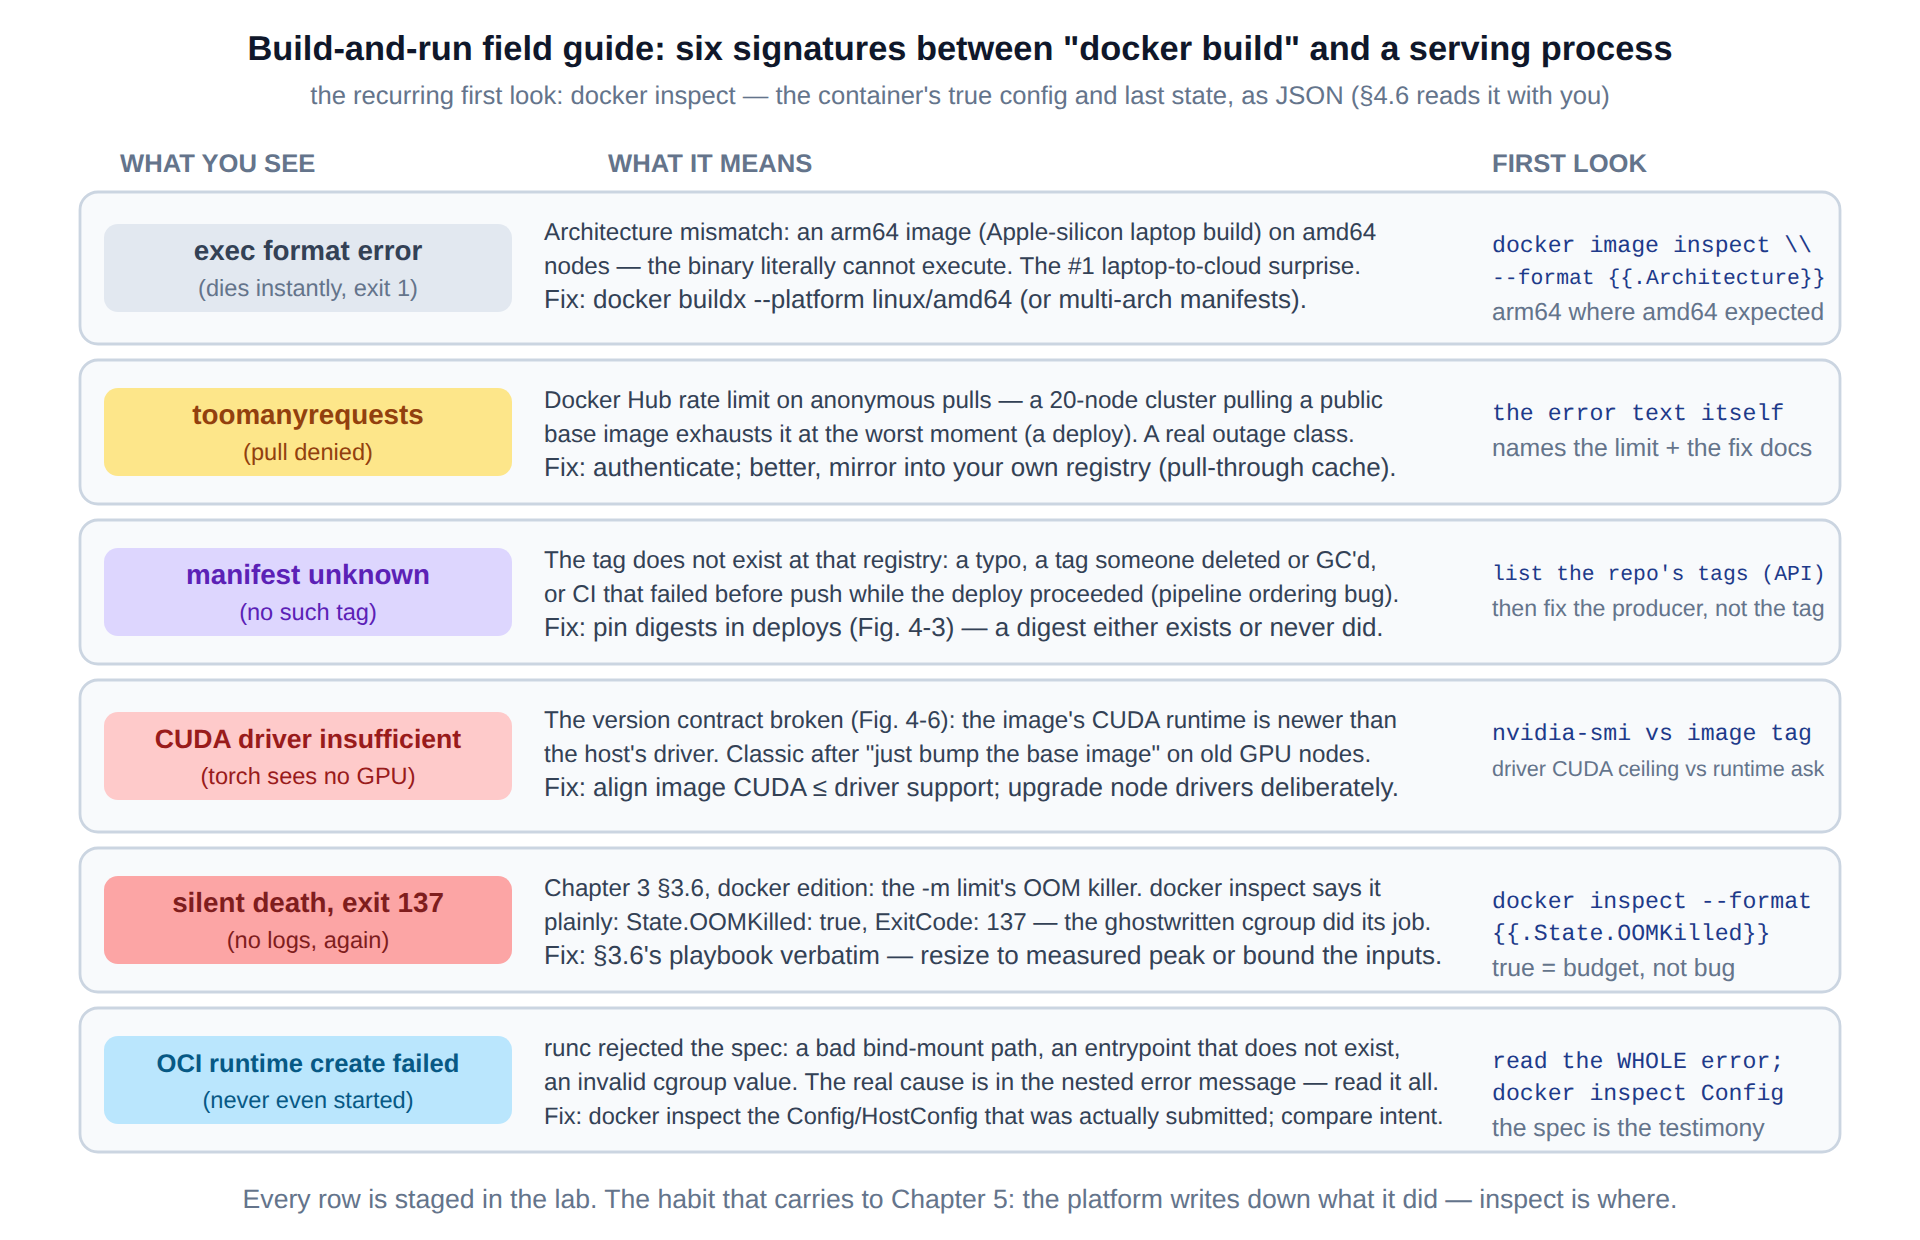
\includegraphics{figures/fig4-7_fieldguide.png}}\\[3pt]
  \figcaption{그림 4-7  빌드와 실행 현장 안내서. 아키텍처 불일치, 속도 제한, 사라진 태그, CUDA 버전 계약, Docker식 OOM, runc의 규격 거부를 각각 첫 명령과 함께 정리한다.}
\end{tbbfigure}

\begin{tbbitemize}
  \item \textbf{즉시 나타나는 exec format error}: 이 CPU에서 바이너리를 실행할 수 없다. Apple Silicon 노트북이 기본으로 만든 arm64 이미지를 amd64 노드에서 실행한 경우다. 2021년 이후 노트북에서 클라우드로 옮길 때 가장 흔한 놀라움이다. \code{docker image inspect --format '\{\{.Architecture\}\}'}로 확인하고 CI의 \code{buildx --platform linux/\allowbreak amd64}로 고치거나 다중 아키텍처를 게시한다. 옆에 \code{no matching manifest for linux/\allowbreak amd64}도 분류하자. 같은 병을 실행 시점이 아니라 pull 시점에 잡은 것이다.
  \item \textbf{pull 중 toomanyrequests}: 플릿이 배포 도중 Docker Hub의 익명 속도 제한을 소진했다. 우선 인증으로 급한 불을 끄고, 장기적으로는 의존하는 공개 베이스를 미러링한다(§4.4). 배포 주기를 제3자의 속도 제한과 결합해서는 안 된다.
  \item \textbf{manifest unknown}: 태그가 없다. 오타, 삭제되었거나 GC된 태그, 빌드가 push하기 전에 배포한 파이프라인이 원인이다. 지속 가능한 해결책은 §4.3의 다이제스트 배포다. 다이제스트는 존재하거나 처음부터 존재하지 않았을 뿐 절반만 push될 수 없다.
  \item \textbf{CUDA driver version is insufficient for CUDA runtime version}: 그림 4-6의 버전 계약을 어겼다. 이미지의 CUDA 사용자 공간이 호스트 드라이버보다 새롭다. 오래된 노드 풀에 "베이스 이미지만 올린" 변경을 배포했을 때 흔하다. 호스트에서 \code{nvidia-smi}가 보여 주는 드라이버/CUDA 상한과 이미지 태그를 비교하고, 우연이 아니라 계획에 따라 드라이버를 올린다.
  \item \textbf{조용한 죽음, exit 137}: 제3장 §3.6을 Docker로 포장한 모습이다. \code{.State.OOMKilled: true}는 \code{-m} 장벽이 강제되었다고 말한다. 측정한 피크에 맞춰 용량을 조정하거나 입력을 제한하는 해법은 같다. 이 플래그는 버그가 아니라 예산 문제였음을 한 명령으로 증명한다.
  \item \textbf{OCI runtime create failed}: 프로세스가 생기기도 전에 runc가 규격을 거부했다. 존재하지 않는 바인드 마운트 원본, 이미지에 없는 엔트리포인트 경로, 잘못된 cgroup 값이 원인일 수 있다. 진짜 원인은 중첩된 오류 가운데 \textit{가장 안쪽}에 있다. 전체 줄을 읽고 \code{docker inspect}로 실제 제출된 Config/HostConfig를 확인해 의도와 비교한다.
\end{tbbitemize}

한 습관이 이 절을 책 전체와 잇는다. \textbf{플랫폼은 자신이 한 일을 기록한다.} 제3장은 커널 장부(\code{/\allowbreak proc}, cgroupfs, dmesg)를 읽었고, 이 절은 런타임 장부(\code{inspect}, \code{events}, \code{logs})를 읽는다. 제5장은 오케스트레이터 장부(describe, events), 제6장은 관문의 장부(상태 코드, 대상 상태)를 읽는다. 네 계층에 규율은 하나다. 장애 대응은 각 계층에 올바른 순서로 증언을 요청하는 연습일 뿐이다.

\begin{calloutbox}{tbbpurple}{tbbpurplefill}
{\normalsize\bfseries\color{tbbpurple}생각해 보기}\par\vspace{3pt}
\begin{tbbitemize}
  \item 컨테이너가 docker run -it에서는 완벽히 실행되지만 Kubernetes에서는 exit 127("not found")로 즉시 죽는다. .Config/.HostConfig 구분을 이용해 대화형 실행과 매니페스트 제출 사이에서 가장 가능성 높은 차이 두 가지를 추론하라. 엔트리포인트 덮어쓰기와 환경 변수 의존 경로를 생각해 보자.
  \item 그림 4-7의 행 가운데 배포 전에 막을 수 있는 모든 실패를 예방하는 다섯 줄짜리 CI 관문을 설계하라. 원칙상 CI에서 잡을 수 없는 두 행은 무엇이며, 각각 어떤 런타임 검사가 대신 다루는가?
  \item docker inspect에는 .HostConfig.Memory = 536870912라고 나오지만 컨테이너가 800 MB를 문제없이 사용한다. 버그라고 부르기 전에 제3장에서 배운 세 가지 설명을 확인 순서대로 나열하라. 실제로 강제하는 cgroup, 페이지 캐시와 익명 메모리의 차이, 실행 중 cgroup을 바꾼 주체를 생각해 보자.
\end{tbbitemize}
\end{calloutbox}

\section{실습: 모델 서버를 컨테이너화하고 push한 뒤 검증하기}

이번 주 실습에서는 이 책의 중심 결과물을 만든다. FastAPI 모델 서버를 잘 설계한 이미지로 만들고 레지스트리에 저장한 뒤 cgroup 파일까지 검증한다. 제5장이 Kubernetes에 배포하고 제6장이 모델 저장소에 연결할 바로 그 이미지다. 모든 작업은 제2장의 VM이나 노트북에서 실행한다. 레지스트리는 무료이고 즉시 실행되며 실제 서비스와 같은 API를 쓰는 로컬 \code{registry:2} 컨테이너다. GPU 부분은 하드웨어가 있는 팀을 위한 선택 부록이다. 제출물은 아래 결과물 체크리스트와 관찰마다 관련 절을 표시한 한 페이지 보고서다.

\subsection*{A부: 제대로 빌드하고 계층의 동작을 증명하기}

\code{serve.py}를 작성한다. 유인물에는 제5장과 제6장에서 프로브할 \code{/\allowbreak predict}, \code{/\allowbreak healthz}, \code{/\allowbreak ready} 엔드포인트를 가진 FastAPI 앱 뼈대가 있다. 두 번 컨테이너화한다. 먼저 단일 단계, 전체 베이스, \code{pip install}보다 앞선 \code{COPY . .}를 쓰는 \textbf{단순 빌드}를 만든다. 다음은 터미널 기록 4-5의 다단계 Dockerfile과 \code{.dockerignore}를 쓴 \textbf{설계 빌드}다. 각각 이미지 크기(\code{docker images}), 계층 지도(\code{docker history}), 순서의 효과를 체감하게 할 측정값인 \textbf{serve.py 한 줄 변경 뒤 재빌드 시간과 "이동할 바이트"}를 기록한다. 둘 다 다시 빌드해 단순 빌드는 pip를 재실행하지만 설계 빌드는 캐시 계층을 모두 재사용해 몇 초 만에 끝나는 모습을 확인한다. \code{docker image inspect --format '\{\{.Architecture\}\}'}로 아키텍처도 명시적으로 확인한다. Apple Silicon 팀은 \code{--platform linux/\allowbreak amd64}를 추가하고 에뮬레이션 비용을 보고서에 적는다.

\subsection*{B부: 실행하고 제한하고 감사하기(강의계획서의 inspect 연습)}

설계 이미지를 실제 예산 \code{-m 512m --cpus 1 -p 8080:8000}으로 실행하고, 자신의 컨테이너에서 터미널 기록 4-8 전체를 재현한다. \code{inspect}로 기록된 의도를 확인하고 \code{/\allowbreak proc/\allowbreak <pid>/\allowbreak cgroup}에서 cgroup 디렉터리로 이동해 \code{memory.max}와 \code{cpu.max}가 플래그와 일치하는 화면을 캡처한다. 이제 제3장이 연 플래그 → 데몬 → containerd → runc → 커널 파일의 고리를 직접 닫았다. 이어 두 가지를 실시간으로 검증한다. \textbf{PID 1 정확성}은 \code{docker stop} 시간을 재서 확인한다. exec 형식 CMD는 SIGTERM을 받아 1초 안에 드레인하고 끝나지만, 의도적으로 만든 셸 형식 버전은 10초의 유예 시간을 꽉 채워 버티다가 SIGKILL된다. 두 시간을 모두 기록한다. \textbf{Docker식 OOM}은 \code{-m 128m}으로 다시 실행해 장난감 추론 루프를 137이 날 때까지 구동한 뒤 \code{.State.OOMKilled: true}를 수집한다. 제3장의 증거 사슬을 이 장의 도구로 확인한 것이다.

\subsection*{C부: 자체 레지스트리에서 프로토콜 관찰하기}

\code{docker run -d -p 5000:5000 --name registry registry:2}를 실행하고 설계 이미지에 태그를 붙여 push한 뒤 계층별 출력을 읽는다. 이어 프로토콜을 가르치는 두 실험을 한다. \textbf{중복 제거}에서는 serve.py 한 줄을 바꾸고 \code{:v2}로 다시 빌드해 push한다. \code{Layer already exists}가 쌓인 가운데 작은 \code{Pushed} 하나만 나오는 화면을 캡처한다. 자신의 터미널 기록 4-6이다. \textbf{다이제스트 규율}에서는 push가 반환한 다이제스트를 각각 기록하고, 다이제스트로 pull한다(\code{docker pull localhost:5000/\allowbreak team/\allowbreak model-server@sha256:...}). 그런 다음 일부러 \code{:v2}를 \textit{다른} 이미지에 다시 붙여 태그는 거짓말할 수 있지만 다이제스트는 그렇지 못함을 증명하고 이를 한 문장 정책으로 쓴다. §6.3의 모델 저장소에서 이미 아는 규칙이 어디서 왔는지 확인하는 순간이다. 마지막으로 현장 안내서의 두 행을 일부러 재현한다. 없는 태그를 pull해 \code{manifest unknown}을 만들고, 팀에 ARM 머신이 있다면 플랫폼을 지정하지 않은 빌드를 x86에서 실행해 \code{exec format error}를 만든다. 화면을 보고서에 넣는다.

\begin{calloutbox}{tbbpurple}{tbbpurplefill}
{\normalsize\bfseries\color{tbbpurple}실습 체크리스트}\par\vspace{3pt}
\begin{tbbitemize}
  \item A부 결과물: 단순형과 설계형의 크기·계층 표, 한 줄 변경 뒤 재빌드 시간 두 개, 아키텍처 확인.
  \item B부 결과물: inspect와 cgroupfs의 일치(자신의 터미널 기록 4-8), exec 형식과 셸 형식의 docker stop 시간, -m 128m에서 OOMKilled: true 캡처.
  \item C부 결과물: 첫 push와 두 번째 push의 기록("Layer already exists"), 다이제스트 pull 증명과 태그 배신 시연, 일부러 재현한 현장 안내서 두 행.
  \item 보고서: 한 페이지. 각 관찰에 관련 절을 적는다. 예: "두 번째 push는 40 KB를 옮겼다. §4.4의 프로토콜이다. 단순 이미지는 1.9 GB를 옮겼을 것이다. §4.3의 순서 역전 때문이다."
  \item 이미지 보관: 최종 빌드에 model-server:v1 태그를 붙이고 디스크가 허용하면 레지스트리를 계속 실행한다. 5주 차 실습에서 바로 이 결과물을 배포한다. 정리해야 한다면 docker rm -f와 docker system prune을 사용하되 먼저 삭제 대상을 읽는다.
\end{tbbitemize}
\end{calloutbox}

\vspace{3.0pt}

\begin{calloutbox}{tbbpurple}{tbbpurplefill}
{\normalsize\bfseries\color{tbbpurple}생각해 보기}\par\vspace{3pt}
\begin{tbbitemize}
  \item B부에서 정지 시간을 재니 exec 형식은 약 0.3 s, 셸 형식은 약 10 s 만에 끝났다. 이 두 숫자를 제5장의 롤링 업데이트와 제6장의 로드 밸런서 드레이닝에 적용하라. Dockerfile 한 줄이 이후 모든 배포에서 사용자에게 어떤 차이를 만드는가?
  \item 실습 레지스트리는 인증도 TLS도 없는 컨테이너 하나다. 프로덕션이라 부르기 전에 더해야 할 항목을 우선순위대로 나열하고, 13주 차 파이프라인이 가장 크게 의존하는 항목도 고르라.
\end{tbbitemize}
\end{calloutbox}

\namedsection{요약}{열 가지로 정리한 제4장}

\qitem{1}{\textbf{프로덕션 컨테이너화는 더 큰 셸 스크립트가 아니라 세 산업적 문제}, 곧 패키징·배포·수명 주기를 푸는 일이다. Docker는 셋을 모두 해결했고 OCI는 그 해법을 누구나 구현할 수 있는 인터페이스로 표준화했다.}

\qitem{2}{\textbf{스택의 각 계층에는 역할이 하나뿐이다.} docker CLI(REST 클라이언트) → dockerd(API와 편의 기능) → containerd(수명 주기 엔진이며 kubelet의 직접 통신 상대) → containerd-shim(컨테이너마다 하나씩 stdio·종료 코드·회수를 담당) → runc(JSON 규격에 따라 제3장의 다섯 단계을 수행한 뒤 종료)로 이어진다. 스택이 모델을 실행하는 것이 아니라 커널이 실행한다.}

\qitem{3}{\textbf{shim은 제3장의 수수께끼 같은 부모 PID 41288을 설명한다.} 가장 작고 지루한 프로그램이 프로세스에 가장 가까이 있으므로 그 위의 모든 구성 요소가 장애·업그레이드·재시작을 겪어도 컨테이너에는 아무 일도 일어나지 않는다.}

\qitem{4}{\textbf{OCI 접합부는 모든 구성 요소를 교체 가능하게 한다.} image-spec은 빌드, distribution-spec은 배포, runtime-spec은 실행을 정의하며 config.json은 제3장을 데이터로 옮긴 것이다. Kata와 gVisor는 런타임 접합부에 들어가고 kubelet은 CRI로 containerd와 직접 통신한다. 2022년 dockershim이 제거되어도 이미지는 신경 쓰지 않았다. Docker 결과물이 아니라 OCI 결과물이기 때문이다.}

\qitem{5}{\textbf{이미지는 콘텐츠 주소 기반 결과물이다.} 매니페스트가 설정과 계층을 가리키며 모든 이름은 sha256이다. 중복 제거, 머신 간 캐시 신뢰, 변조 탐지가 이름에서 자연스럽게 나온다. 태그는 움직일 수 있는 별명이므로 배포는 다이제스트를 고정한다. §6.3 모델 저장소의 불변성 규율도 여기서 배웠다.}

\qitem{6}{\textbf{Dockerfile은 이 책의 누적된 교훈을 빌드에 얼려 넣은 파일이다.} 변경 빈도에 따른 순서(제3장의 캐시), 코드보다 앞선 requirements(순서가 뒤집히면 재빌드에 20분), .dockerignore, 다단계 빌드(빌드 의존성은 실행 페이로드가 아니다: 2.4 GB→610 MB, cuda-devel→cuda-runtime: 9.8 GB→3.1 GB), exec 형식 CMD(PID 1, 제3·5·6장에서 보상), 비루트 USER를 적용한다.}

\qitem{7}{\textbf{레지스트리는 없는 다이제스트만 움직인다.} 중복 제거는 최적화가 아니라 프로토콜이다. 따뜻한 플릿의 코드 배포는 KB만 움직이지만 새 노드와 풀 폭풍은 GB를 움직인다(12주 차의 콜드 스타트 세금). 풀 시크릿/IAM으로 인증하고, 속도 제한이 장애가 되지 않도록 공개 베이스를 미러링하며, GC와 스캐닝을 적용한다(13주 차의 관문).}

\qitem{8}{\textbf{GPU는 패키징하지 않고 주입한다.} 이미지는 CUDA 사용자 공간을, 호스트는 커널 모듈과 버전이 맞는 드라이버 사용자 공간을 담는다. NVIDIA 툴킷의 OCI 훅이 생성 시점에 장치 노드·바인드 마운트 라이브러리·NVIDIA\_VISIBLE\_DEVICES로 둘을 결합한다. 디바이스 플러그인은 같은 메커니즘 위에 클러스터 재고와 할당을 더한다(제5장의 정수 리소스).}

\qitem{9}{\textbf{커널이 GPU 연산을 볼 수 없으므로 cgroup은 이를 스케줄링할 수 없다.} 작업은 드라이버가 관리하는 명령 대기열로 들어가며 사용자 공간에 매핑되어 시스템 호출조차 없을 수 있다. 커널에는 장치 파일만 있고 연산 단위는 없다. cgroup의 역할은 접근 통제뿐이고 공유는 공급업체 메커니즘에 있다(제2장). VRAM 고갈은 커널 OOM이 아니라 잡을 수 있는 할당자 OOM이다.}

\qitem{10}{\textbf{docker inspect는 런타임의 선서 증언이다.} State는 OOMKilled와 ExitCode 등 종료 방식을, Config와 HostConfig는 이미지의 의도와 운영자의 의도를, GraphDriver는 제3장의 overlay 디렉터리를, RootFS.Layers는 실제 실행 중인 바이트를 보여 준다. 현장 안내서의 여섯 징후인 exec format error, toomanyrequests, manifest unknown, CUDA driver insufficient, 조용한 137, OCI runtime create failed에는 각각 첫 명령이 있고 실습에서 직접 재현한다.}

\namedsection{연습문제}{}

\subsection*{A. 객관식}

\qitem{1}{model-server 컨테이너 30개가 실행 중인 노드에서 Docker 데몬을 재시작했다. 컨테이너에는 무슨 일이 일어나며, 그 이유는 무엇인가?}

\begin{tbboptions}
  \item ① dockerd가 부모이므로 모두 재시작한다.
  \item ② PID 1의 자식인 장기 실행 containerd-shim이 각각 붙들고 있으므로 아무 영향 없이 계속 실행한다.
  \item ③ 데몬이 돌아올 때까지 일시 정지한다.
  \item ④ 계속 실행하지만 네트워크 네임스페이스를 잃는다.
\end{tbboptions}

\qitem{2}{runc에 관한 설명으로 옳은 것은?}

\begin{tbboptions}
  \item ① 각 컨테이너 옆에서 상주 감독자로 실행된다.
  \item ② Kubernetes가 CRI로 통신하는 데몬이다.
  \item ③ OCI runtime-spec의 config.json을 읽고 네임스페이스/cgroup/rootfs를 설정해 프로세스를 시작한 뒤 종료한다.
  \item ④ 서로 다른 아키텍처 사이에서 이미지를 변환한다.
\end{tbboptions}

\qitem{3}{serve.py 한 줄을 바꿔 다시 빌드하고 push했다. 계층 순서가 올바르면 약 40 KB만 움직이는 이유는?}

\begin{tbboptions}
  \item ① 레지스트리가 다른 계층을 압축해 없애기 때문이다.
  \item ② push가 다이제스트로 협상하며 바뀌지 않은 모든 계층은 레지스트리에 "이미 존재"하므로 새 코드 계층만 업로드하기 때문이다.
  \item ③ Docker가 소스 트리의 차이를 계산해 패치를 보내기 때문이다.
  \item ④ 태그가 포인터이므로 어떤 데이터도 두 번 움직이지 않기 때문이다.
\end{tbboptions}

\qitem{4}{Apple Silicon 노트북에서 만든 이미지가 클라우드 노드에서 "exec format error"와 함께 즉시 죽었다. 원인과 해결책은?}

\begin{tbboptions}
  \item ① push가 손상되었다. 다시 push한다.
  \item ② CUDA 버전이 맞지 않는다. 드라이버 버전을 맞춘다.
  \item ③ amd64 노드에 arm64 이미지를 배포했다. CI에서 --platform linux/amd64로 빌드하거나 다중 아키텍처를 만든다.
  \item ④ 실행 권한이 없다. Dockerfile에서 chmod +x를 실행한다.
\end{tbboptions}

\qitem{5}{이미지는 CUDA 런타임을 담지만 NVIDIA 드라이버 라이브러리는 절대 담지 않는 이유는?}

\begin{tbboptions}
  \item ① 라이선스가 재배포를 금지하기 때문이다.
  \item ② 드라이버 사용자 공간은 호스트 커널 모듈과 정확히 맞아야 하므로 생성 시 호스트에서 주입한다. 이미지에 넣으면 드라이버 업그레이드 때 깨진다.
  \item ③ 드라이버가 이미지 계층에 넣기에는 너무 크기 때문이다.
  \item ④ 드라이버는 C로 작성되었고 이미지는 Python만 담기 때문이다.
\end{tbboptions}

\qitem{6}{로그 없이 컨테이너가 죽었다. docker inspect에 ExitCode: 137, OOMKilled: true가 나온다. 올바른 해석은?}

\begin{tbboptions}
  \item ① 커널 OOM 킬러가 -m 상한을 강제했다(제3장 §3.6). 측정한 피크에 맞춰 늘리거나 입력을 제한한다.
  \item ② 애플리케이션이 세그멘테이션 오류로 죽었다.
  \item ③ 이미지가 비정상이어서 Docker가 종료했다.
  \item ④ 레지스트리가 이미지를 회수했다.
\end{tbboptions}

\subsection*{B. 단답형}

\qitem{1}{docker CLI → dockerd → containerd → shim → runc 사슬에서 각 구성 요소의 단 하나뿐인 역할을 쓰고, 실행 중인 컨테이너의 프로세스 트리에 없는 두 구성 요소와 그 이유를 설명하라.}

\qitem{2}{태그와 다이제스트를 각각 정의하고, 태그로 배포할 때의 실패 모드를 제시하며, 이 책이 한 계층 위에서 같은 불변성 규율을 적용하는 두 곳을 쓰라.}

\qitem{3}{NVIDIA Container Toolkit이 컨테이너 생성 시 수행하는 세 가지 주입을 나열하고, 그중 cgroup이 관여하는 항목과 제한된 역할을 설명하라.}

\qitem{4}{팀 이미지가 9.8 GB(cuda-devel, 단일 단계, COPY 순서 역전)다. 약 3.1 GB이면서 코드 배포는 KB 단위가 되게 하는 세 변경과 각각 구현하는 장의 교훈을 쓰라.}

\subsection*{C. 서술형}

\qitem{1}{"Docker가 오래 남긴 공헌은 데몬이 아니라 규격이다." shim 아키텍처, dockershim 제거, 런타임 접합부(Kata/gVisor)를 근거로 이 주장에 찬성하거나 반박하라. 이미지와 런타임이 한 공급업체의 독점 기술로 남았다면 ML 서빙이 어떻게 달라졌을지도 논하라.}

\qitem{2}{팀 엔지니어링 안내서의 "이미지 표준" 절을 작성하라. 베이스 이미지 정책(slim/runtime 대 devel), 계층 순서, 다단계 빌드, USER/CMD, 아키텍처, 태그/다이제스트 정책과 각각을 강제하는 CI 관문을 포함하고, 모든 규칙을 이 장 또는 제3·5·6장의 실패나 비용으로 정당화하라.}

\qitem{3}{GPU 이야기는 네 장에 걸쳐 이어진다(§4.5의 상자). 새 동료를 위해 하나의 일관된 글로 다시 설명하라. 커널이 GPU 연산을 스케줄링하지 못하는 이유, 그 결과 공급업체가 맡게 된 일(제2장), 패키징에 생긴 요구(이 장), 오케스트레이션에 생긴 요구(제5장)를 인과 관계로 연결하고, 12주 차의 공유 결정에 미칠 영향으로 마무리하라.}

\namedsection{정답과 해설}{}

\subsection*{A. 객관식}

\qitem{1}{\textbf{②} shim은 실행 중에 데몬이 하중을 떠받치는 부품이 되지 않게 하려고 존재한다. PID 1의 자식으로 stdio와 종료 코드를 붙든다. 터미널 기록 4-2에서 데몬 재시작으로 직접 증명했다. (§4.2)}

\qitem{2}{\textbf{③} runc는 상주 프로그램이 아니라 설치 작업반이다. config.json에 따라 다섯 단계을 수행한 뒤 종료한다. ②는 CRI 통신 상대인 containerd와 혼동했다. (§4.2)}

\qitem{3}{\textbf{②} 중복 제거가 곧 프로토콜이다. push는 "없는 다이제스트가 무엇인가?"라고 묻는다. 순서가 올바르면 40 KB 코드 계층만 새롭다. ③처럼 소스 차이를 보내는 것이 아니며 단위는 차이가 아니라 계층이다. (§4.3–4.4)}

\qitem{4}{\textbf{③} 아키텍처 불일치는 노트북에서 클라우드로 옮길 때 가장 흔한 문제다. 바이너리를 실행할 수 없어 애플리케이션 코드에 도달하기 전에 죽는다. --platform은 CI가 책임져야 한다. (§4.4, §4.6)}

\qitem{5}{\textbf{②} 호스트마다 커널 모듈과 드라이버 사용자 공간의 버전이 서로 고정되어 있다. 툴킷이 생성 시 호스트의 라이브러리를 바인드 마운트하므로 드라이버를 올려도 이미지는 이식성을 유지한다. (§4.5)}

\qitem{6}{\textbf{①} 137 + OOMKilled: true는 제3장의 장벽에 Docker의 서류가 붙은 것이다. 버그가 아니라 예산 문제다. 피크를 측정해 크기를 조정하거나 입력을 제한하는 절차는 같다. (§3.6, §4.6)}

\subsection*{B. 단답형}

\qitem{1}{CLI는 REST 클라이언트다. dockerd는 개발자 API, 빌드, 편의 기능을 맡는다. containerd는 이미지·스냅숏·작업의 수명 주기를 관리하며 CRI를 통한 kubelet의 통신 상대다. shim은 컨테이너별 stdio·종료 코드·회수를 장기간 맡는다. runc는 config.json의 다섯 단계을 수행하고 종료한다. 프로세스 트리에 없는 것은 dockerd와 runc다. dockerd는 처음부터 조상이 아니며 shim은 PID 1의 자식이 되고, runc는 설정 뒤 종료한다. (§4.2)}

\qitem{2}{다이제스트는 매니페스트의 sha256 정체로 구조상 불변이다. 태그는 이름→다이제스트를 잇는 가변 포인터다. 태그가 이동하거나 다시 push되면 노드와 시간에 따라 "v2"가 다른 바이트를 뜻해 감사 기록이 사라지고 캐시가 오염된다. 한 계층 위의 같은 규율은 §6.3 모델 저장소 버전(새 버전 = 새 접두사, sha256 매니페스트)과 13주 차 다이제스트 승격 파이프라인에 적용된다. (§4.3, §6.3)}

\qitem{3}{(1) \code{/dev/nvidia*} 장치 노드를 컨테이너에 넣고 cgroup \textit{장치 허용 규칙}으로 접근을 통제한다. 이것이 유일한 cgroup 역할이다. (2) nvidia.ko와 맞아야 하는 호스트 드라이버 사용자 공간 라이브러리를 바인드 마운트한다. (3) NVIDIA\_VISIBLE\_DEVICES로 컨테이너에 보일 GPU를 선택한다. 목록 어디에도 스케줄링은 없다. 바로 그 점이 핵심이다. (§4.5)}

\qitem{4}{(1) 최종 단계를 cuda:-runtime으로 한 다단계 빌드로 약 7 GB devel 도구 모음을 뺀다. 빌드 의존성은 실행 페이로드가 아니다. (2) requirements+설치를 코드 COPY보다 앞에 두어 제3장의 캐시 경제성을 적용한다. 코드 배포가 의존성 계층을 더는 무효화하지 않는다. (3) .dockerignore로 컨텍스트를 정리하고 제6장에 따라 가중치를 이미지에서 뺀다. 결과는 약 3.1 GB 이미지와 약 40 KB 배포다. (§4.3)}

\subsection*{C. 서술형(채점 기준)}

\qitem{1}{강한 찬성 답안은 shim/데몬 분리로 데몬을 교체 가능한 존재로 만든 점(Docker 자체 구성 요소도 특권적이지 않음), dockershim 제거라는 자연 실험(생태계가 데몬을 버려도 결과물은 그대로), Kata/gVisor를 받아들이는 런타임 접합부(제2장의 스펙트럼이 설정 한 줄이 됨)를 든다. 반사실적 상황에서는 공급업체 종속 이미지가 캐시/중복 제거의 경제성을 분열시키고 §4.4의 레지스트리 상호운용성을 막아 Kubernetes 생태계 자체를 늦추었을 가능성을 논한다. 반박은 데몬 시대의 사용성이 보급을 이끌었고 표준은 성공 뒤에 왔다고 지적할 수 있다. 어느 입장이든 논증을 평가한다. (§4.2)}

\qitem{2}{근거가 붙은 규칙을 찾는다. devel이 아닌 runtime(9.8 GB → 3.1 GB, §4.3), 순서+.dockerignore(20분 재빌드, KB 배포), 컴파일 의존성의 다단계 빌드 의무화, exec 형식 CMD+비루트 USER(제3·5·6장의 보상), CI의 --platform(exec format error), 배포의 다이제스트 또는 불변 태그(manifest unknown, 감사)가 포함되어야 한다. CI 관문으로 두 아키텍처 빌드, 크기 예산, 스캔, push 후 배포 순서, 다이제스트 승격을 제시한다. 공개 베이스 미러 정책(속도 제한)은 가산점이다. (§4.3–4.6)}

\qitem{3}{점수를 줄 핵심 흐름은 다음과 같다. 커널은 볼 수 있는 것만 스케줄링한다. GPU 작업은 커널에 보이지 않는 드라이버 관리 대기열로 들어간다 → cgroup 컨트롤러가 존재할 수 없다(제3장의 공백을 메커니즘으로 설명) → 공유는 공급업체 계층의 시간 분할/MPS/MIG가 맡아야 했다(제2장) → 패키징은 드라이버(호스트)와 CUDA 사용자 공간(이미지)을 나누고 주입으로 결합해야 했다(이 장) → 오케스트레이션은 정수만 약속할 수 있다(제5장) → 12주 차의 공유 결정은 공급업체 메커니즘 하나를 고르고 격리 절충을 받아들이는 일이다. 목록만 아니라 인과 화살표가 있어야 만점이다. (§4.5)}

\namedsection{더 읽을거리}{}

\textbf{[이번 주]} 표시는 지금 읽어야 할 필수 자료이고, \textbf{[N주 차]} 표시는 해당 주에 도움이 될 자료다.

\begin{tbbitemize}
  \item \textbf{[이번 주] Marc Levinson, "The Box: How the Shipping Container Made the World Smaller and the World Economy Bigger" (2006), 1장}: §4.1 사례 B의 실제 역사다. 재래식 하역의 경제성, 맥린, Ideal-X, 표준화의 정치를 다룬다. §4.1은 단순한 비유가 아니라 계보이며, 이 책에서 가장 재미있는 필수 읽을거리다.
  \item \textbf{[이번 주] OCI runtime-spec과 image-spec (opencontainers.org)}: 제3장에서는 config.json을 한 번 훑었다. 이제 모국어처럼 읽어 보자. image-spec의 매니페스트 절은 10분이면 읽고 §4.3의 내용을 오래 남게 한다.
  \item \textbf{[이번 주] Docker 문서: "Dockerfile best practices"와 BuildKit 문서}: 공급업체가 설명하는 §4.3이다. 캐시 마운트, 다단계 패턴, 빌드 비밀을 다룬다. 자격 증명을 이미지에 굽지 않는 규칙은 제6장의 키 없는 규칙을 빌드 시점에 적용한 것이다.
  \item \textbf{[이번 주] NVIDIA Container Toolkit 문서("How it works")}: §4.5의 주입 메커니즘을 원 출처에서 설명하며 생태계가 표준화 중인 CDI(Container Device Interface) 방향도 포함한다.
  \item \textbf{containerd 문서: 아키텍처와 스냅쇼터}: 수명 주기 엔진이 이미지와 제3장의 overlay 스택을 모델링하는 법을 다룬다. 지연 로딩 스냅쇼터 절은 12주 차 콜드 스타트의 최전선이다.
  \item \textbf{Kubernetes 디바이스 플러그인 문서}: 제5장의 정수 리소스 뒤에 있는 gRPC 계약이다. 짧으면서 §4.5와 §5.5의 고리를 닫는다.
  \item \textbf{[5주 차] Kubernetes 문서: "Images"(imagePullPolicy, 풀 시크릿)}: 이 장의 레지스트리 규율이 연결되는 kubelet 쪽 설정이다.
  \item \textbf{[12주 차] 이미지 스트리밍/사전 pull에 관한 클라우드 공급업체 문서와 "690 ms cold starts" 같은 엔지니어링 글}: §4.4의 풀 폭풍 문제를 산업 규모로 확장한 사례다.
  \item \textbf{[13주 차] Sigstore/cosign과 SLSA 개요}: 파이프라인에 공급망 보안이 들어올 때 "다이제스트를 신뢰하라"가 서명과 출처 증명으로 자라는 모습을 다룬다.
\end{tbbitemize}

\vspace{5.0pt}

\begin{calloutbox}{tbbblue}{tbbbluefill}
{\normalsize\bfseries\color{tbbblue}다음 장: 제5장 Kubernetes}\par\vspace{3pt}
이제 레지스트리에 저장된 잘 만든 이미지를 손에 넣었고 GPU 접근도 주입 훅까지 이해했다. 한 번의 \code{docker run}으로 머신 한 대에서 서비스할 수 있다. 다음 주에는 플릿으로 간다. 원하는 상태를 영원히 조정하므로 다시는 서버를 직접 "시작"하지 않는다는 Kubernetes의 핵심 생각, 이를 구현하는 구조와 CRI를 통해 이 장의 containerd를 구동하는 kubelet, 서빙의 삼위일체인 Pod / Deployment / Service, 플릿 규모에서 제3장의 cgroup 파일을 대필하는 리소스 requests와 limits, 비싼 GPU를 정수·테인트(taint)·빈 패킹(bin packing)으로 배치하는 스케줄러를 배운다. 실습에서는 이번 주에 push한 바로 그 이미지를 minikube 클러스터에 배포하고 노출한 뒤 여섯 방식으로 망가뜨려 각 징후로 진단한다. 인프라 이야기가 완성되기까지 이제 한 장 남았다.
\end{calloutbox}
